\chapter{Réalisation}

Ce dernier chapitre est celui où la conception prend enfin forme concrète. J’y présente l’environnement de travail utilisé, les interfaces réellement développées et fonctionnelles, la démarche de test suivie, ainsi que certaines difficultés rencontrées en cours de route et la façon dont je les ai résolues.

\section{Introduction}
\label{sec_4_1}
Toutes les captures d’écran qui suivent proviennent de l’application en fonctionnement, pas de maquettes : chaque interface présentée a été testée et utilisée pendant le stage.

\section{Environnement de travail}
\label{sec_4_2}
\subsection{Environnement matériel}
\label{sec_4_2_1}
J’ai réalisé le développement sur un poste de travail standard mis à disposition par l’entreprise, doté d’un processeur multi-cœurs et d’une mémoire vive suffisante pour faire tourner simultanément l’environnement de développement, le serveur back-end, le serveur front-end, la base de données PostgreSQL et le serveur n8n en local.

\subsection{Environnement logiciel}
\label{sec_4_2_2}
Les outils et technologies suivants ont été mobilisés tout au long du projet :

\begin{itemize}
\item Langages : Java 17, TypeScript, HTML5, SCSS, SQL.
\item Frameworks et bibliothèques : Spring Boot 3 (Web, Data JPA, Security), Angular 20, Bootstrap.
\item Base de données : PostgreSQL, administrée via pgAdmin.
\item Automatisation et IA : n8n (agents d’automatisation par webhooks), API de Cohere (scoring IA des CV). Assistant conversationnel candidat : API OpenRouter (modèle z-ai/glm-5.3-flash, format compatible OpenAI).
\item Environnements de développement intégrés : Eclipse STS (Spring Tool Suite) pour le développement back-end Java/Spring Boot, Visual Studio Code pour le développement front-end Angular.
\item Modélisation UML : StarUML pour la conception des diagrammes de cas d’utilisation, de classes et de séquence présentés aux chapitres 2 et 3 ; le rendu graphique des figures a été produit avec PlantUML à partir de la description textuelle de ces modèles.
\item Gestion de version : Git, hébergement du code sur GitHub.
\item Outils de test et de documentation d’API : Postman pour les tests manuels des API REST, Swagger (springdoc-openapi) pour la documentation interactive générée automatiquement.
\item Build et gestion de dépendances : Maven pour le back-end, npm pour le front-end.
\end{itemize}

\subsection{Gestion de version}
\label{sec_4_2_3}
J’ai organisé le versionnement du code autour d’une branche principale, avec des messages de commit descriptifs qui facilitent la traçabilité des évolutions fonctionnelles et des corrections apportées tout au long du stage.

\subsection{Sécurité applicative}
\label{sec_4_2_4}
Plusieurs mécanismes concrets protègent la plateforme et les données des candidats. Les mots de passe ne sont jamais stockés en clair : ils sont hachés avec BCrypt avant persistance. L’authentification s’appuie sur un jeton JWT signé \cite{ref14}, valable 24 heures, transmis à chaque requête et vérifié côté back-end pour en extraire l’identité et les rôles de l’utilisateur. Chaque point d’entrée de l’API REST est protégé par annotation selon le rôle requis (@PreAuthorize), et un contrôle d’accès supplémentaire restreint, pour un manager, la visibilité aux seuls candidats de son périmètre — déterminé prioritairement par son département, la famille de métier ne servant de repli que pour les offres non rattachées à un département. Le dépôt de CV est limité aux formats PDF, DOC et DOCX, avec une taille maximale de 10 Mo côté API, resserrée à 5 Mo par la validation du formulaire Angular, pour limiter les risques liés au téléversement de fichiers. Des mécanismes complémentaires, comme l’analyse antivirus ou une validation plus poussée du contenu au-delà de la seule extension et du type MIME, pourraient compléter ce dispositif en production, conformément aux recommandations de l’OWASP \cite{ref15}.

\section{Interfaces graphiques de l’application}
\label{sec_4_3}
Cette section présente les interfaces de la plateforme, regroupées par acteur : l’accès public et l’espace candidat (figures~\ref{fig_4_1} à \ref{fig_4_5}), l’espace RH et le suivi du processus de recrutement (figures~\ref{fig_4_6} à \ref{fig_4_14}), l’espace manager (figures~\ref{fig_4_15a}, \ref{fig_4_15b} et \ref{fig_4_16}), l’espace administrateur et la traçabilité (figures~\ref{fig_4_17} à \ref{fig_4_19}), enfin la chaîne d’automatisation n8n (figures~\ref{fig_4_20} à \ref{fig_4_22}). Toutes ces captures proviennent de l’application en fonctionnement. Les captures pleine page sont présentées en paysage : à contenu identique, c’est ce qui fait passer leur texte d’environ 5 pt à 7 pt imprimés, et les plus chargées ont en outre été recadrées pour atteindre 8 à 9 pt.

\subsection{Accès public et espace candidat}
\label{sec_4_3_1}
% figure 4.1
\setcounter{figure}{0}
\begin{sidewaysfigure}
\centering
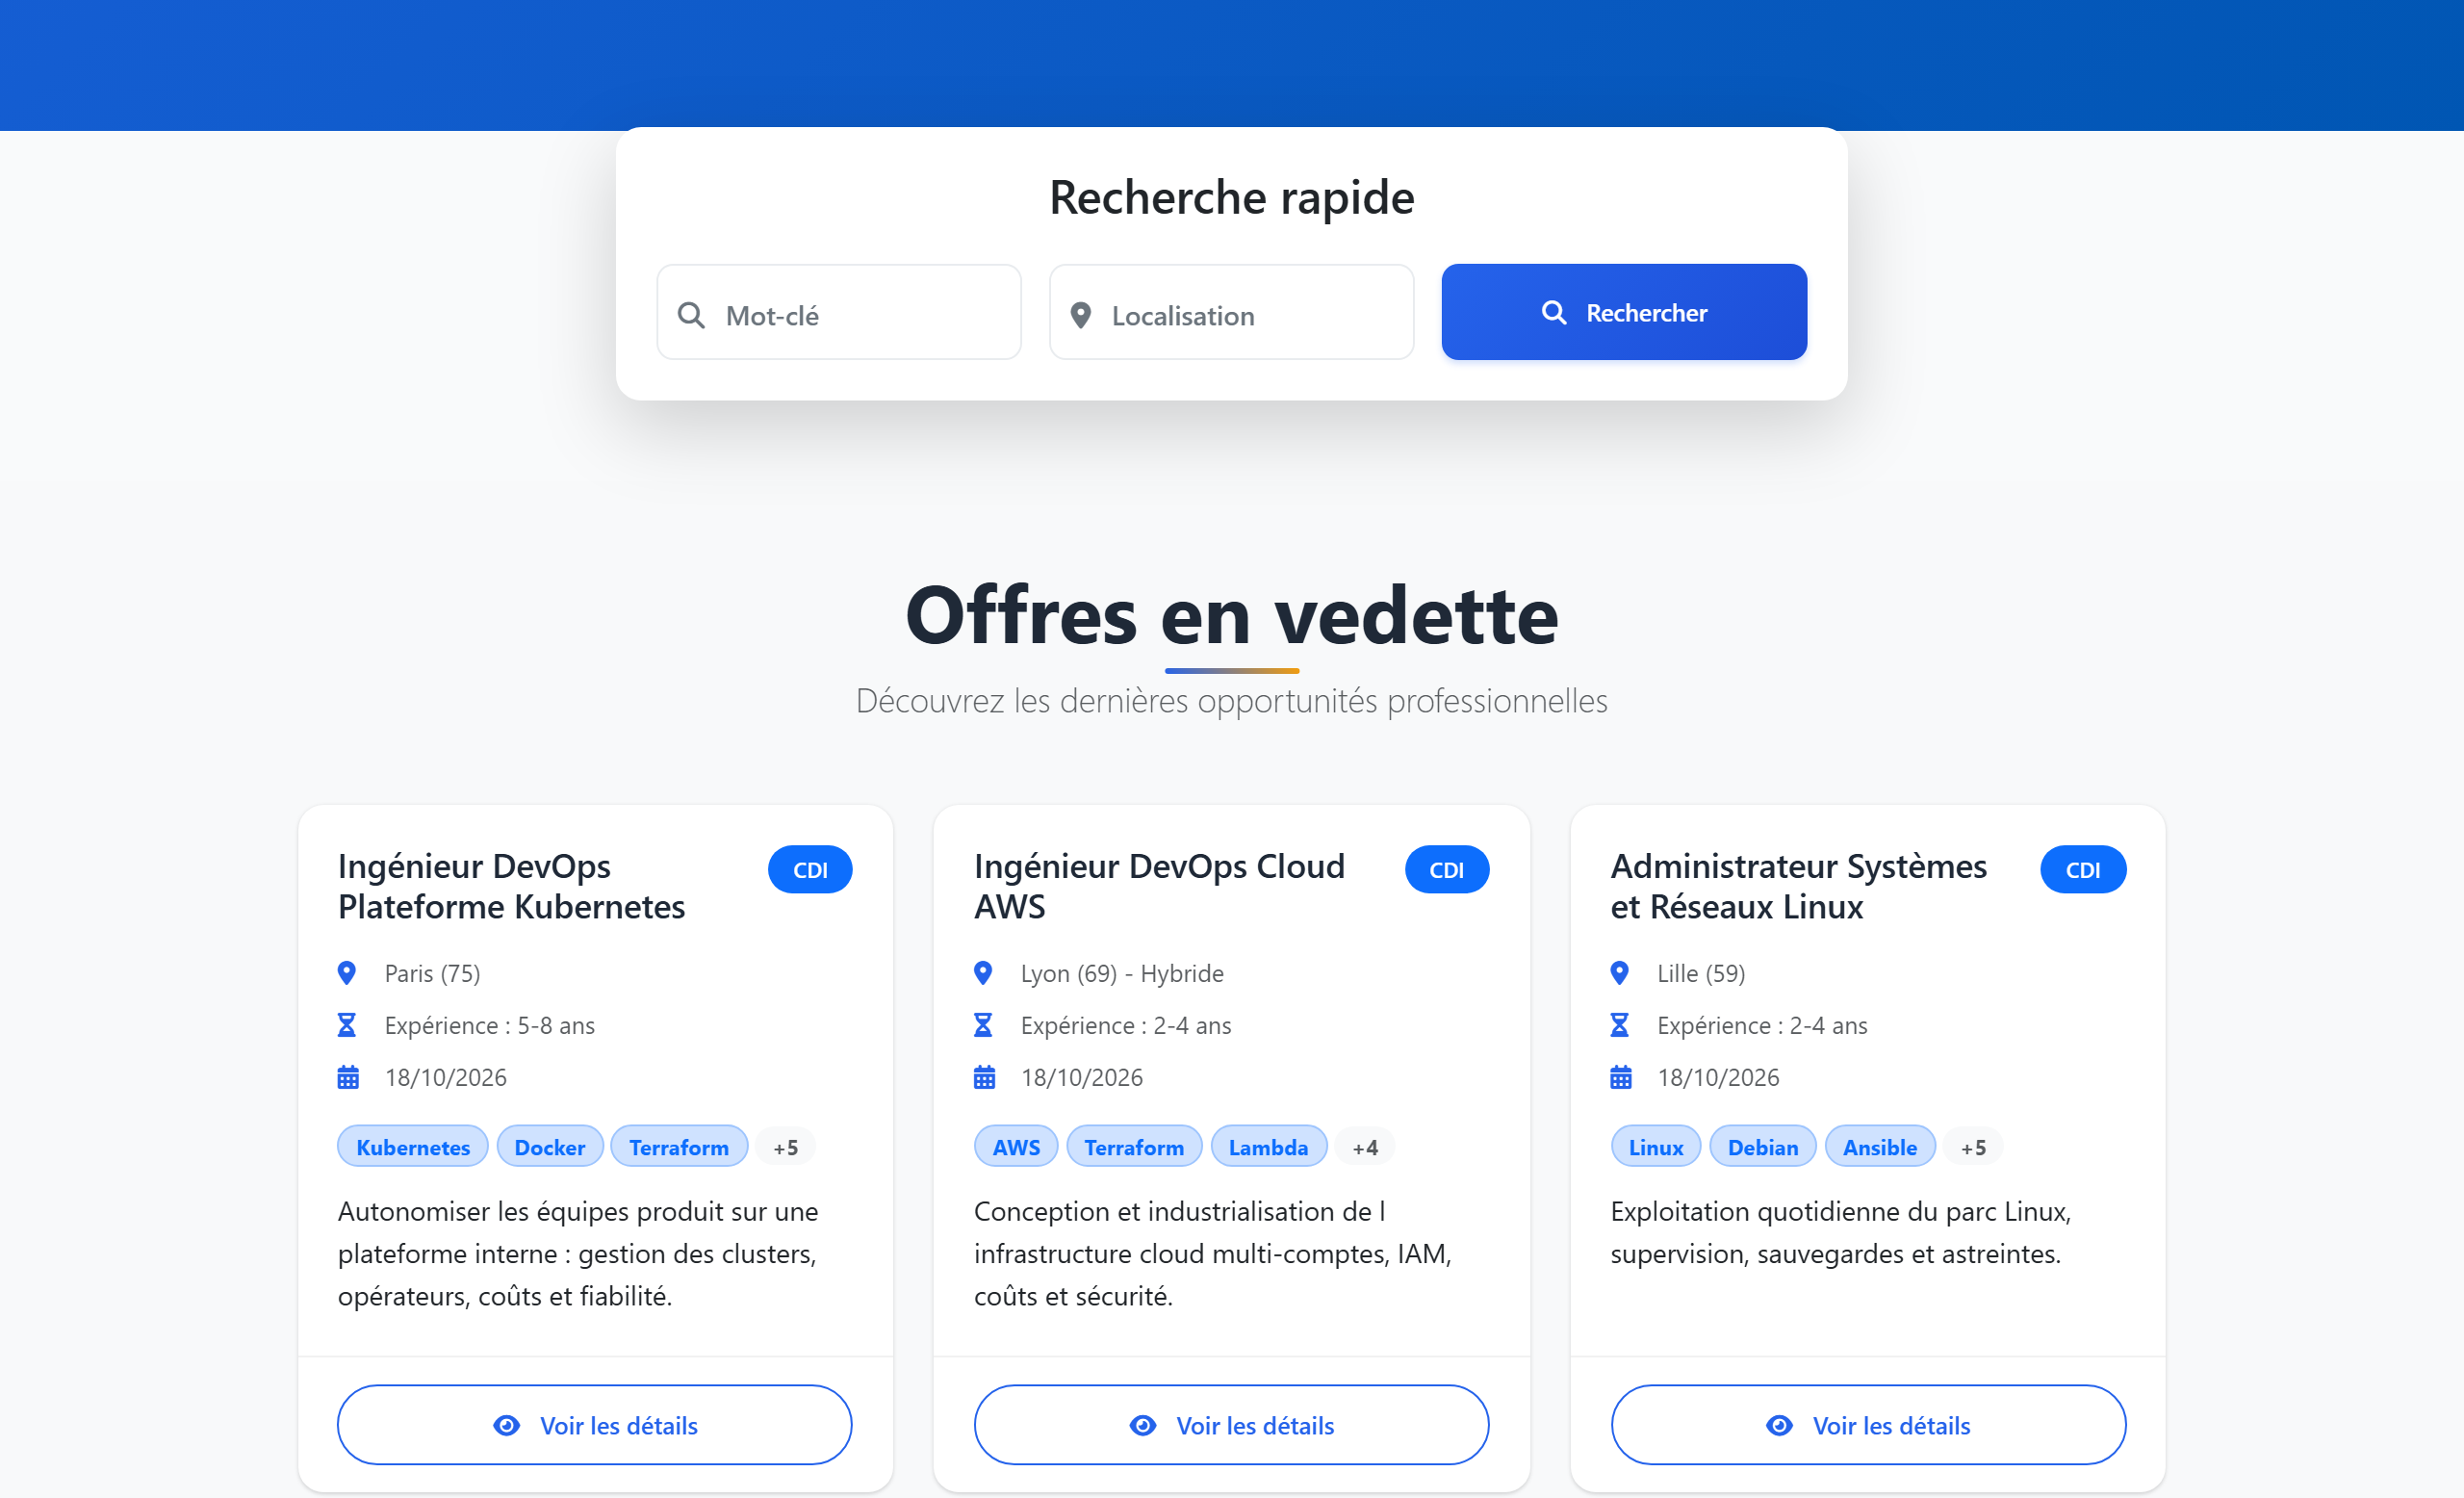
\includegraphics[width=0.98\textheight, height=0.62\textheight, keepaspectratio]{fig4_1}
\caption{Page d’accueil publique — recherche d’offres d’emploi}
\label{fig_4_1}
\end{sidewaysfigure}

Accessible sans authentification, la page d’accueil de la figure~\ref{fig_4_1} propose un cartouche de « Recherche rapide » par mot-clé et par localisation et présente, sous le titre « Offres en vedette » — « Découvrez les dernières opportunités professionnelles » —, les offres les plus récemment publiées : chaque carte porte l’intitulé du poste, son type de contrat, son lieu, l’expérience demandée, ses compétences clés, sa date de publication, un extrait de la description et un bouton « Voir les détails ».

% figure 4.2
\setcounter{figure}{1}
\begin{figure}[!ht]
\centering

\includegraphics[width=\textwidth, height=0.80\textheight, keepaspectratio]{fig4_2}
\caption{Page de connexion}
\label{fig_4_2}
\end{figure}

La page de connexion de la figure~\ref{fig_4_2} est le point d’entrée des espaces sécurisés : l’authentification s’y fait par nom d’utilisateur et mot de passe, et le jeton JWT renvoyé par le back-end sécurise ensuite l’ensemble des requêtes vers l’API.

% figure 4.3
\setcounter{figure}{2}
\begin{figure}[!ht]
\centering
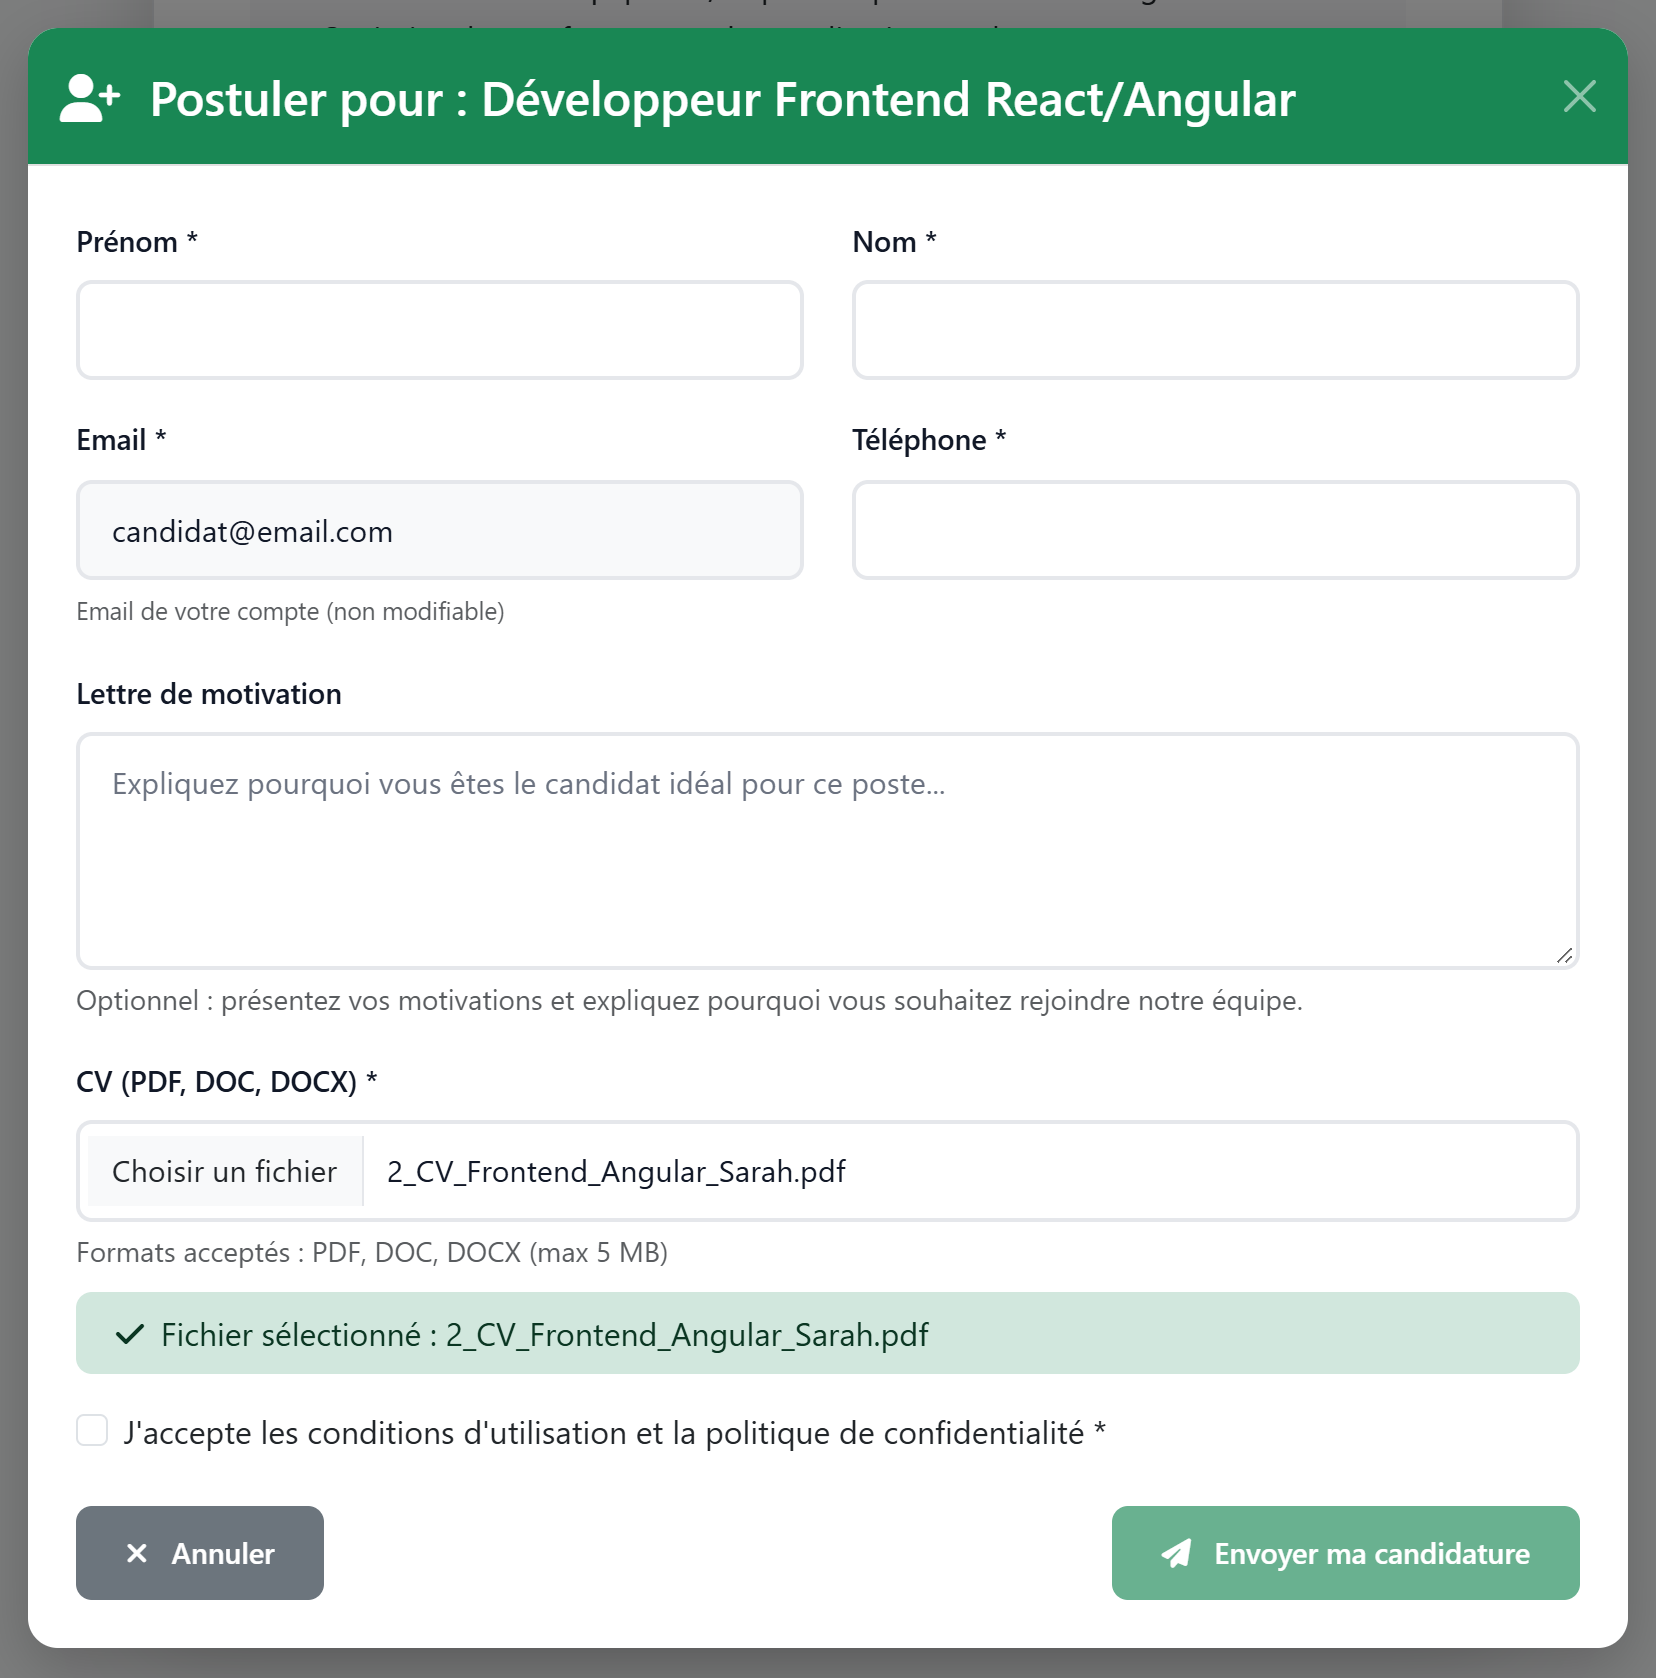
\includegraphics[width=\textwidth, height=0.80\textheight, keepaspectratio]{fig4_3}
\caption{Soumission d’une candidature avec dépôt de CV}
\label{fig_4_3}
\end{figure}

Comme le montre la figure~\ref{fig_4_3}, un candidat connecté postule directement depuis une offre : le formulaire pré-remplit son e-mail de compte, valide le format du CV (PDF, DOC, DOCX) et confirme visuellement la sélection avant l’envoi. C’est ce dépôt qui déclenche la chaîne décrite en section~\ref{sec_3_5_3} (extraction du texte par l’agent n8n, analyse par l’API de Cohere appelée par le back-end, score automatique).

% figure 4.4
\setcounter{figure}{3}
\begin{sidewaysfigure}
\centering
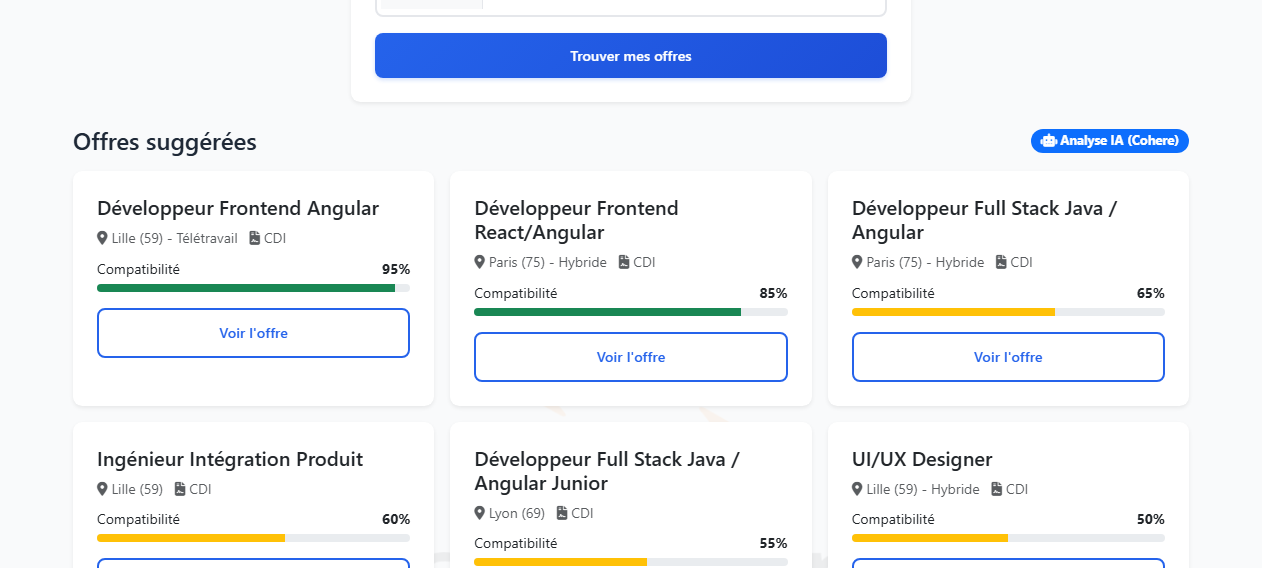
\includegraphics[width=0.98\textheight, height=0.62\textheight, keepaspectratio]{fig4_4}
\caption{Fonctionnalité « Job idéal » — suggestions d’offres selon le CV}
\label{fig_4_4}
\end{sidewaysfigure}

Comme l’illustre la figure~\ref{fig_4_4}, un visiteur ou un candidat qui ne postule à aucune offre précise peut déposer son CV et recevoir une liste des offres actives classées par pourcentage de compatibilité, calculée par l’API de Cohere (badge « Analyse IA (Cohere) », avec repli automatique sur un classement par mots-clés si l’IA est indisponible).

% figure 4.5
\setcounter{figure}{4}
\begin{figure}[!ht]
\centering
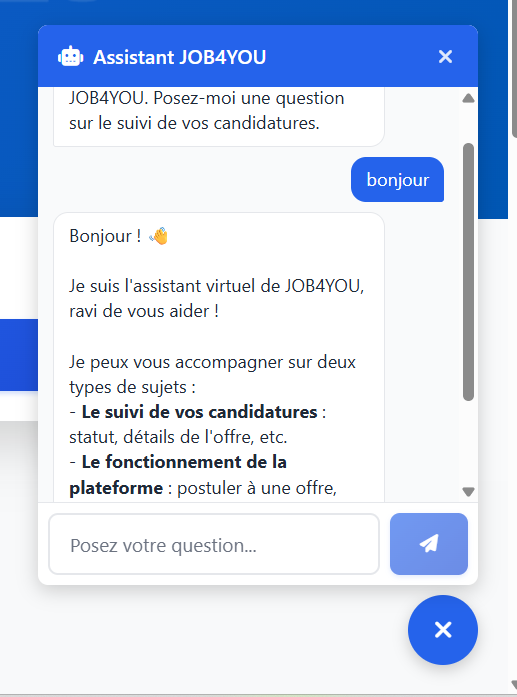
\includegraphics[width=\textwidth, height=0.80\textheight, keepaspectratio]{fig4_5}
\caption{Assistant conversationnel candidat (chatbot)}
\label{fig_4_5}
\end{figure}

Disponible uniquement pour un candidat authentifié, le widget de la figure~\ref{fig_4_5} permet de poser des questions en langage naturel sur le suivi de ses propres candidatures ou sur le fonctionnement général de la plateforme (offres, Job idéal, retrait de candidature, etc.). Les réponses sont générées par un modèle de raisonnement (z-ai/glm-5.3-flash, via l’API OpenRouter) à partir d’un contexte constitué côté serveur par une liste blanche de champs : intitulé du poste, libellé du statut, date de candidature, entretiens et, le cas échéant, les feedbacks explicitement transmis au candidat. Les champs internes (score et résumé générés par l’agent de scoring, correction manuelle du RH, identité de l’intervieweur, notes internes d’entretien) n’entrent pas dans cette liste et ne quittent donc pas le back-end vers le prompt ; ce filtre structurel, complété par les consignes du message système, a été vérifié sur les scénarios testés, y compris une tentative d’injection de prompt.

\subsection{Espace RH — suivi du processus de recrutement}
\label{sec_4_3_2}
% figure 4.6
\setcounter{figure}{5}
\begin{sidewaysfigure}
\centering
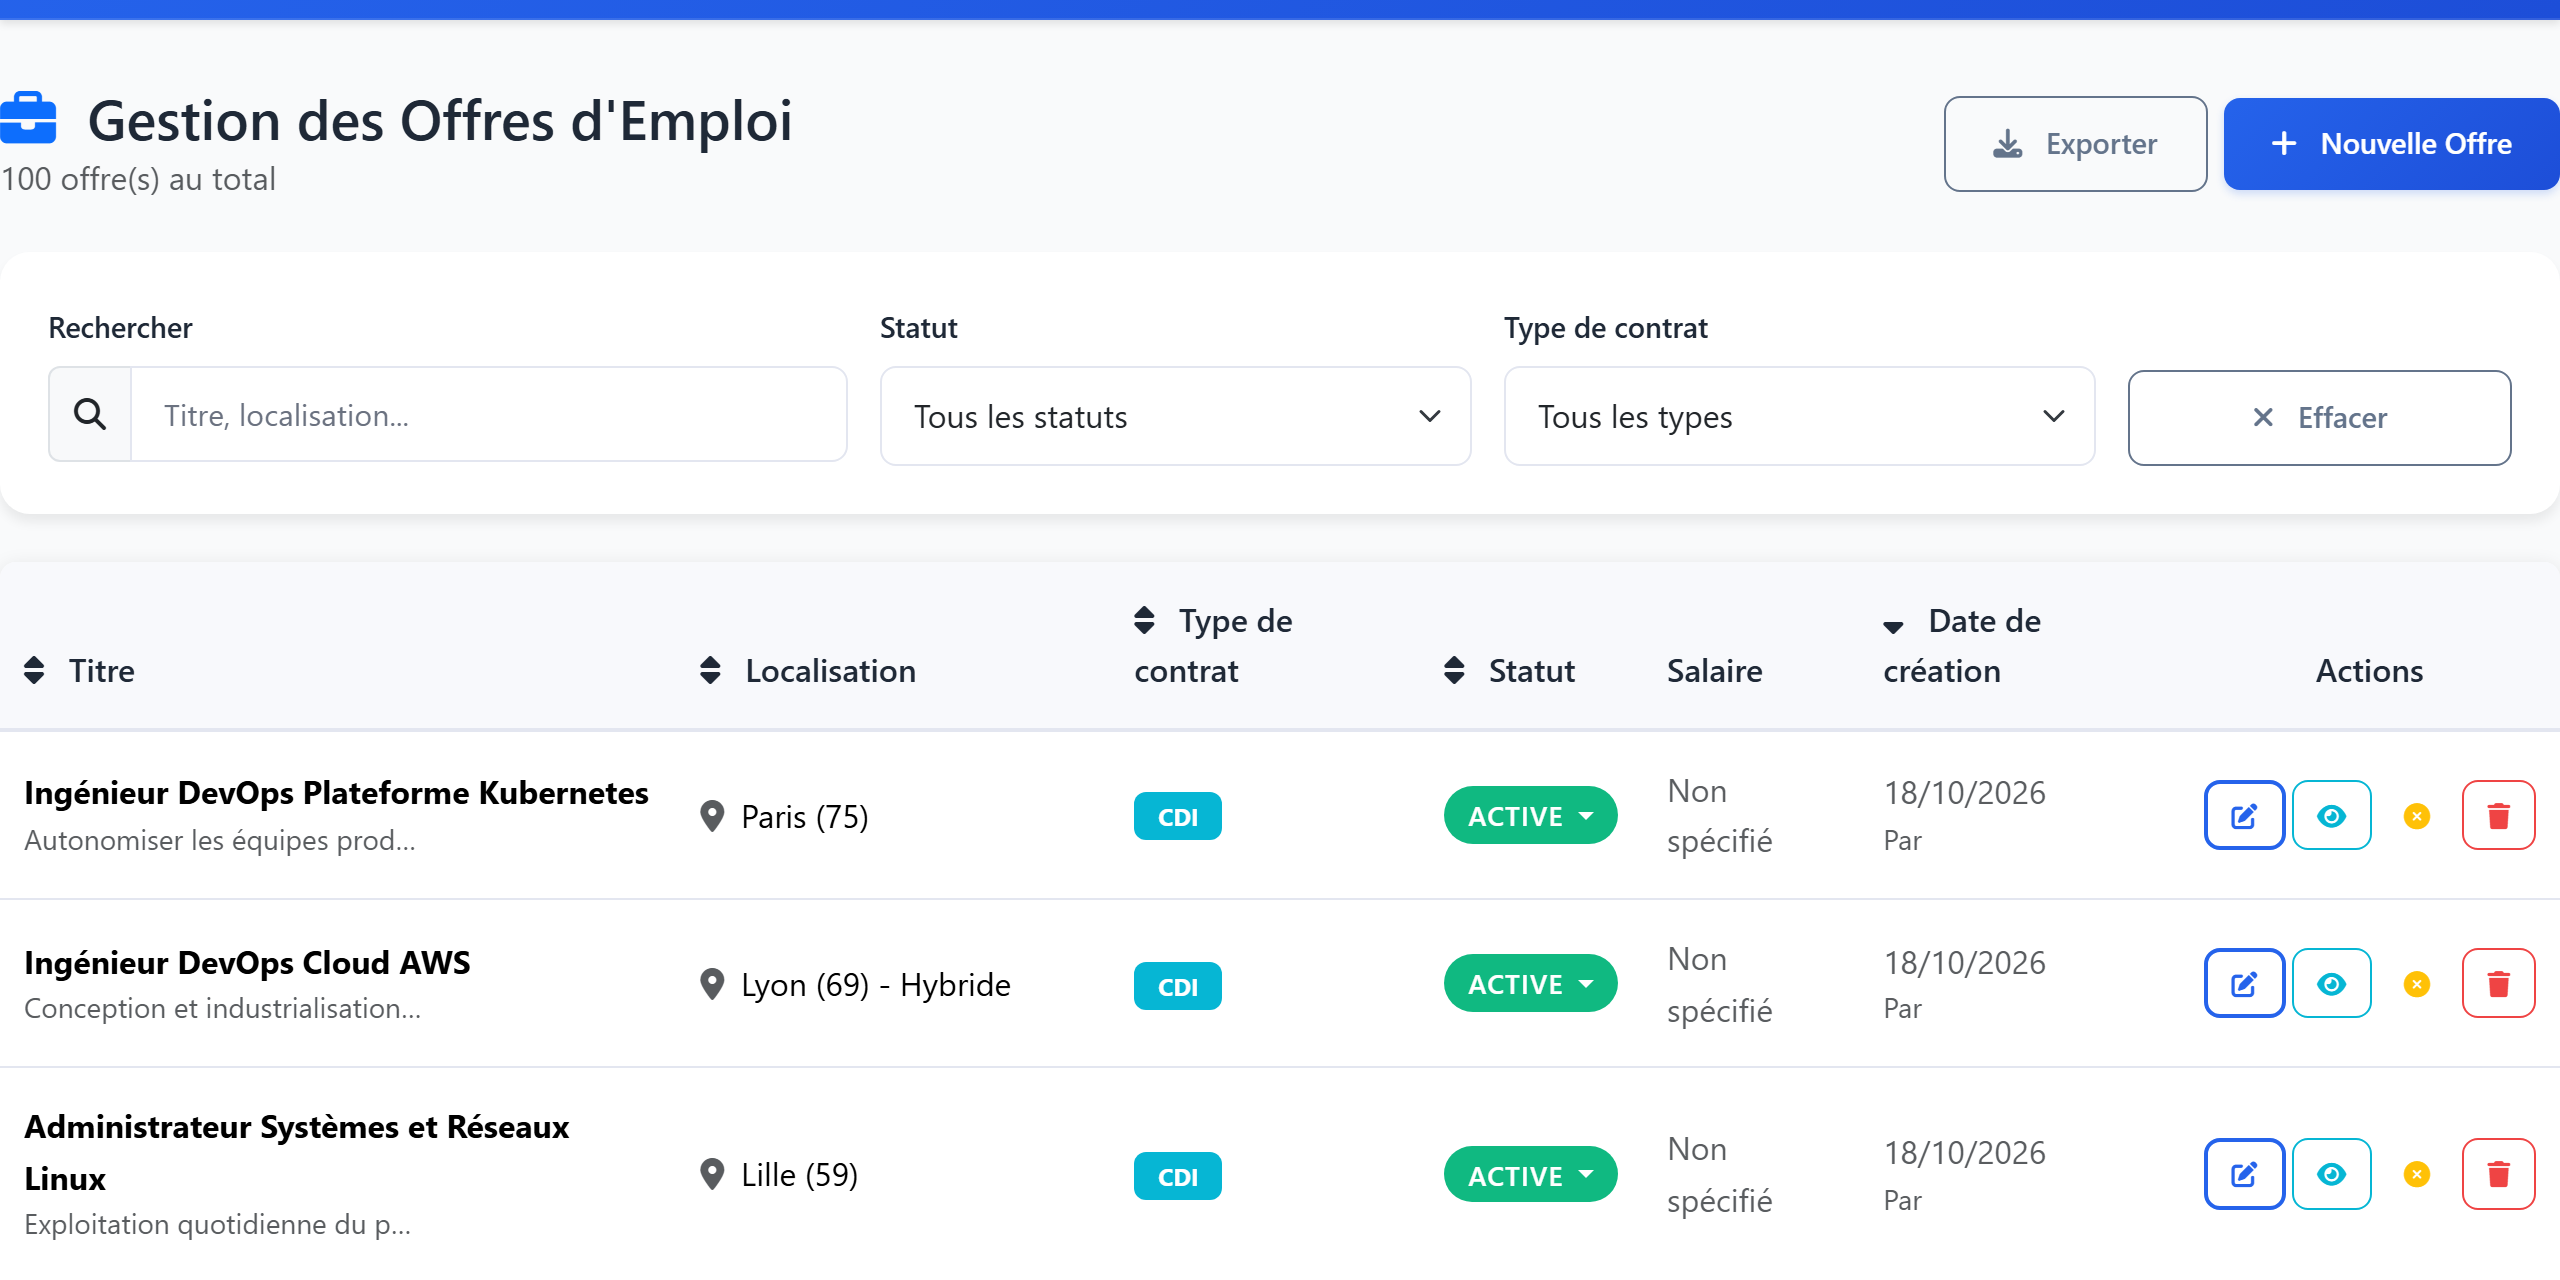
\includegraphics[width=0.98\textheight, height=0.62\textheight, keepaspectratio]{fig4_6}
\caption{Gestion des offres d’emploi (espace RH)}
\label{fig_4_6}
\end{sidewaysfigure}

Comme le montre la figure~\ref{fig_4_6}, le responsable RH crée, modifie et suit le statut de chaque offre depuis une table filtrable par mot-clé, par statut et par type de contrat, avec un accès direct à la consultation, à la modification et à la suppression ; la bascule en « expirée » se fait automatiquement une fois la date limite dépassée.

% figure 4.7
\setcounter{figure}{6}
\begin{sidewaysfigure}
\centering
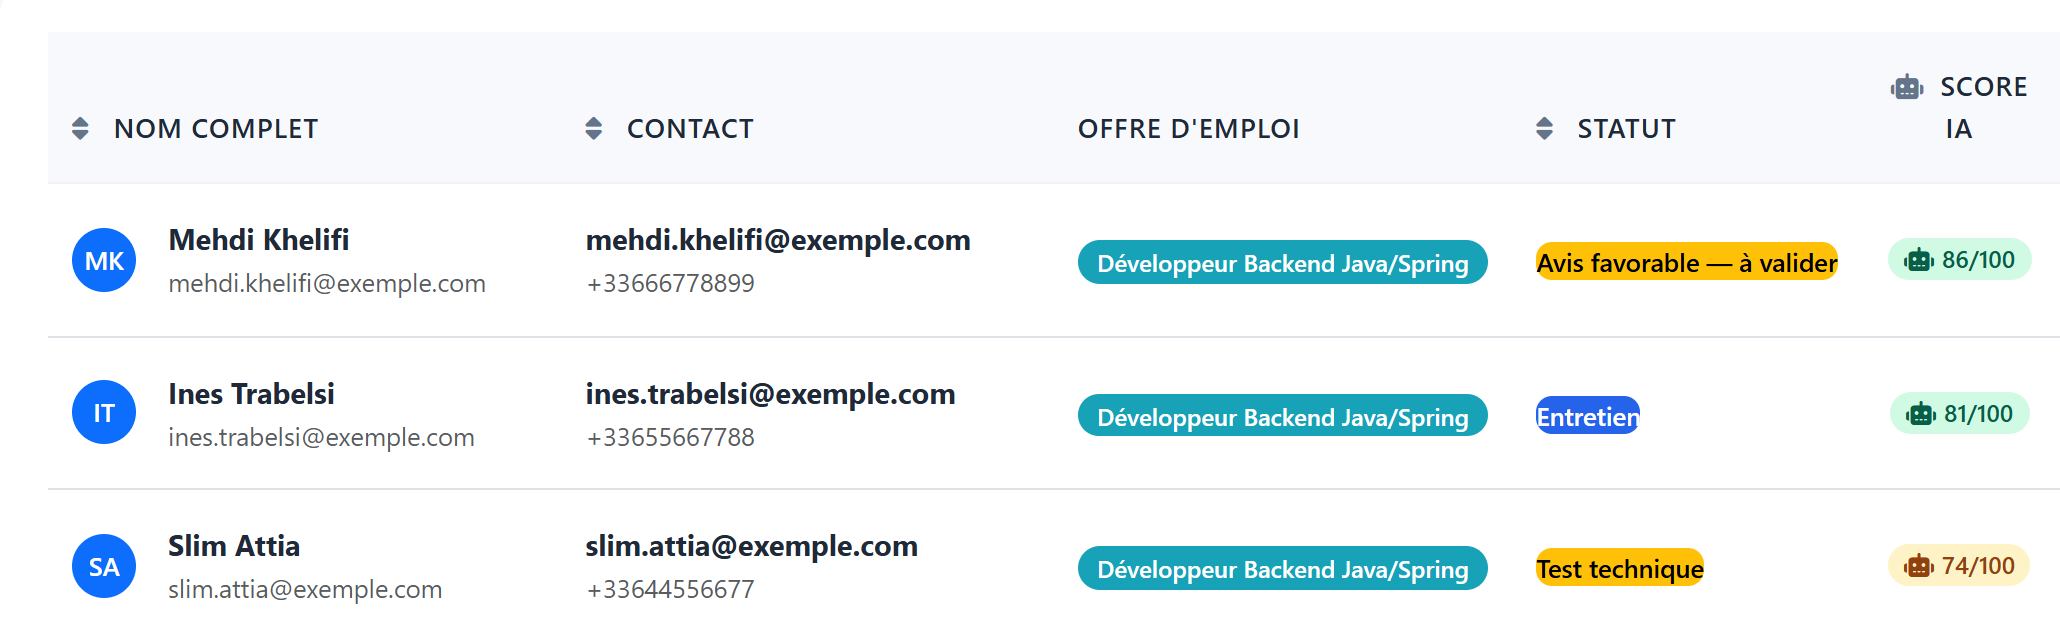
\includegraphics[width=0.98\textheight, height=0.62\textheight, keepaspectratio]{fig4_7}
\caption{Gestion des candidats — vue liste avec score IA}
\label{fig_4_7}
\end{sidewaysfigure}

La figure~\ref{fig_4_7} reproduit la liste des dossiers de l’espace RH : pour chacun apparaissent le contact, l’offre visée, le statut courant et le score de l’agent IA — coloré selon son niveau. Une colonne d’actions rapides accompagne par ailleurs chaque ligne (consultation en ligne du CV, téléchargement, modification, envoi d’e-mail, suppression), et le bandeau supérieur résume l’état du vivier par quatre compteurs cliquables — « À valider », « Rejetés », « Retirées », « Embauchés » — qui basculent la liste sur le filtre correspondant ; ces deux zones, situées en haut et à droite de l’écran, ne sont pas reproduites sur le recadrage, qui privilégie la lisibilité du tableau.

% figure 4.8
\setcounter{figure}{7}
\begin{figure}[!ht]
\centering
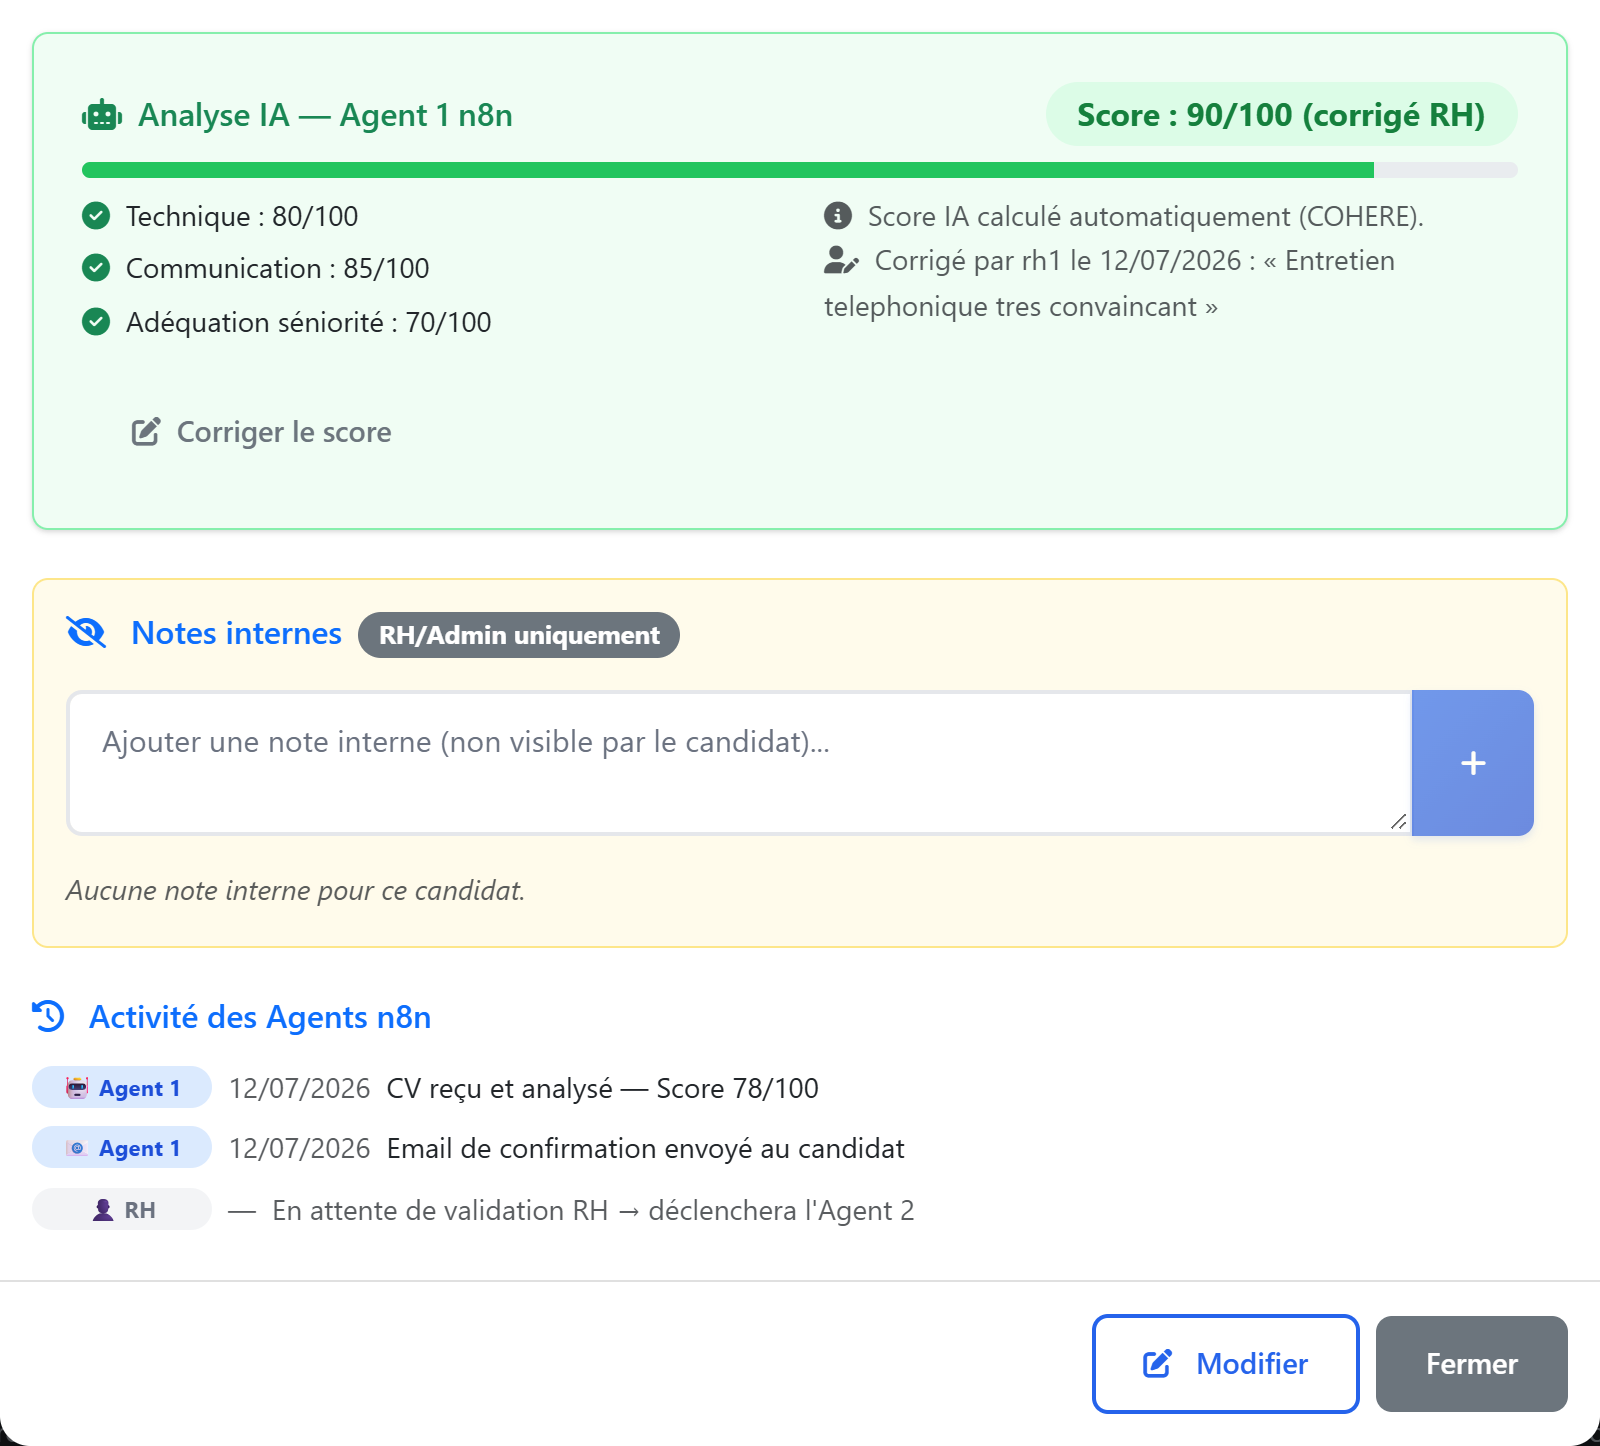
\includegraphics[width=\textwidth, height=0.80\textheight, keepaspectratio]{fig4_8}
\caption{Analyse détaillée d’une candidature par intelligence artificielle}
\label{fig_4_8}
\end{figure}

Le détail d’une candidature, reproduit en figure~\ref{fig_4_8}, expose, au-delà du score global visible en liste (figure~\ref{fig_4_7}), la répartition par critère — technique, communication, adéquation séniorité —, le bouton « Corriger le score » et, le cas échéant, la correction manuelle appliquée par un RH avec sa justification, conformément au principe de contrôle humain décrit en section~\ref{sec_4_6}. Y figurent également les notes internes, réservées aux rôles RH et administrateur, et l’activité des agents n8n sur le dossier.

% figure 4.9
\setcounter{figure}{8}
\begin{figure}[!ht]
\centering
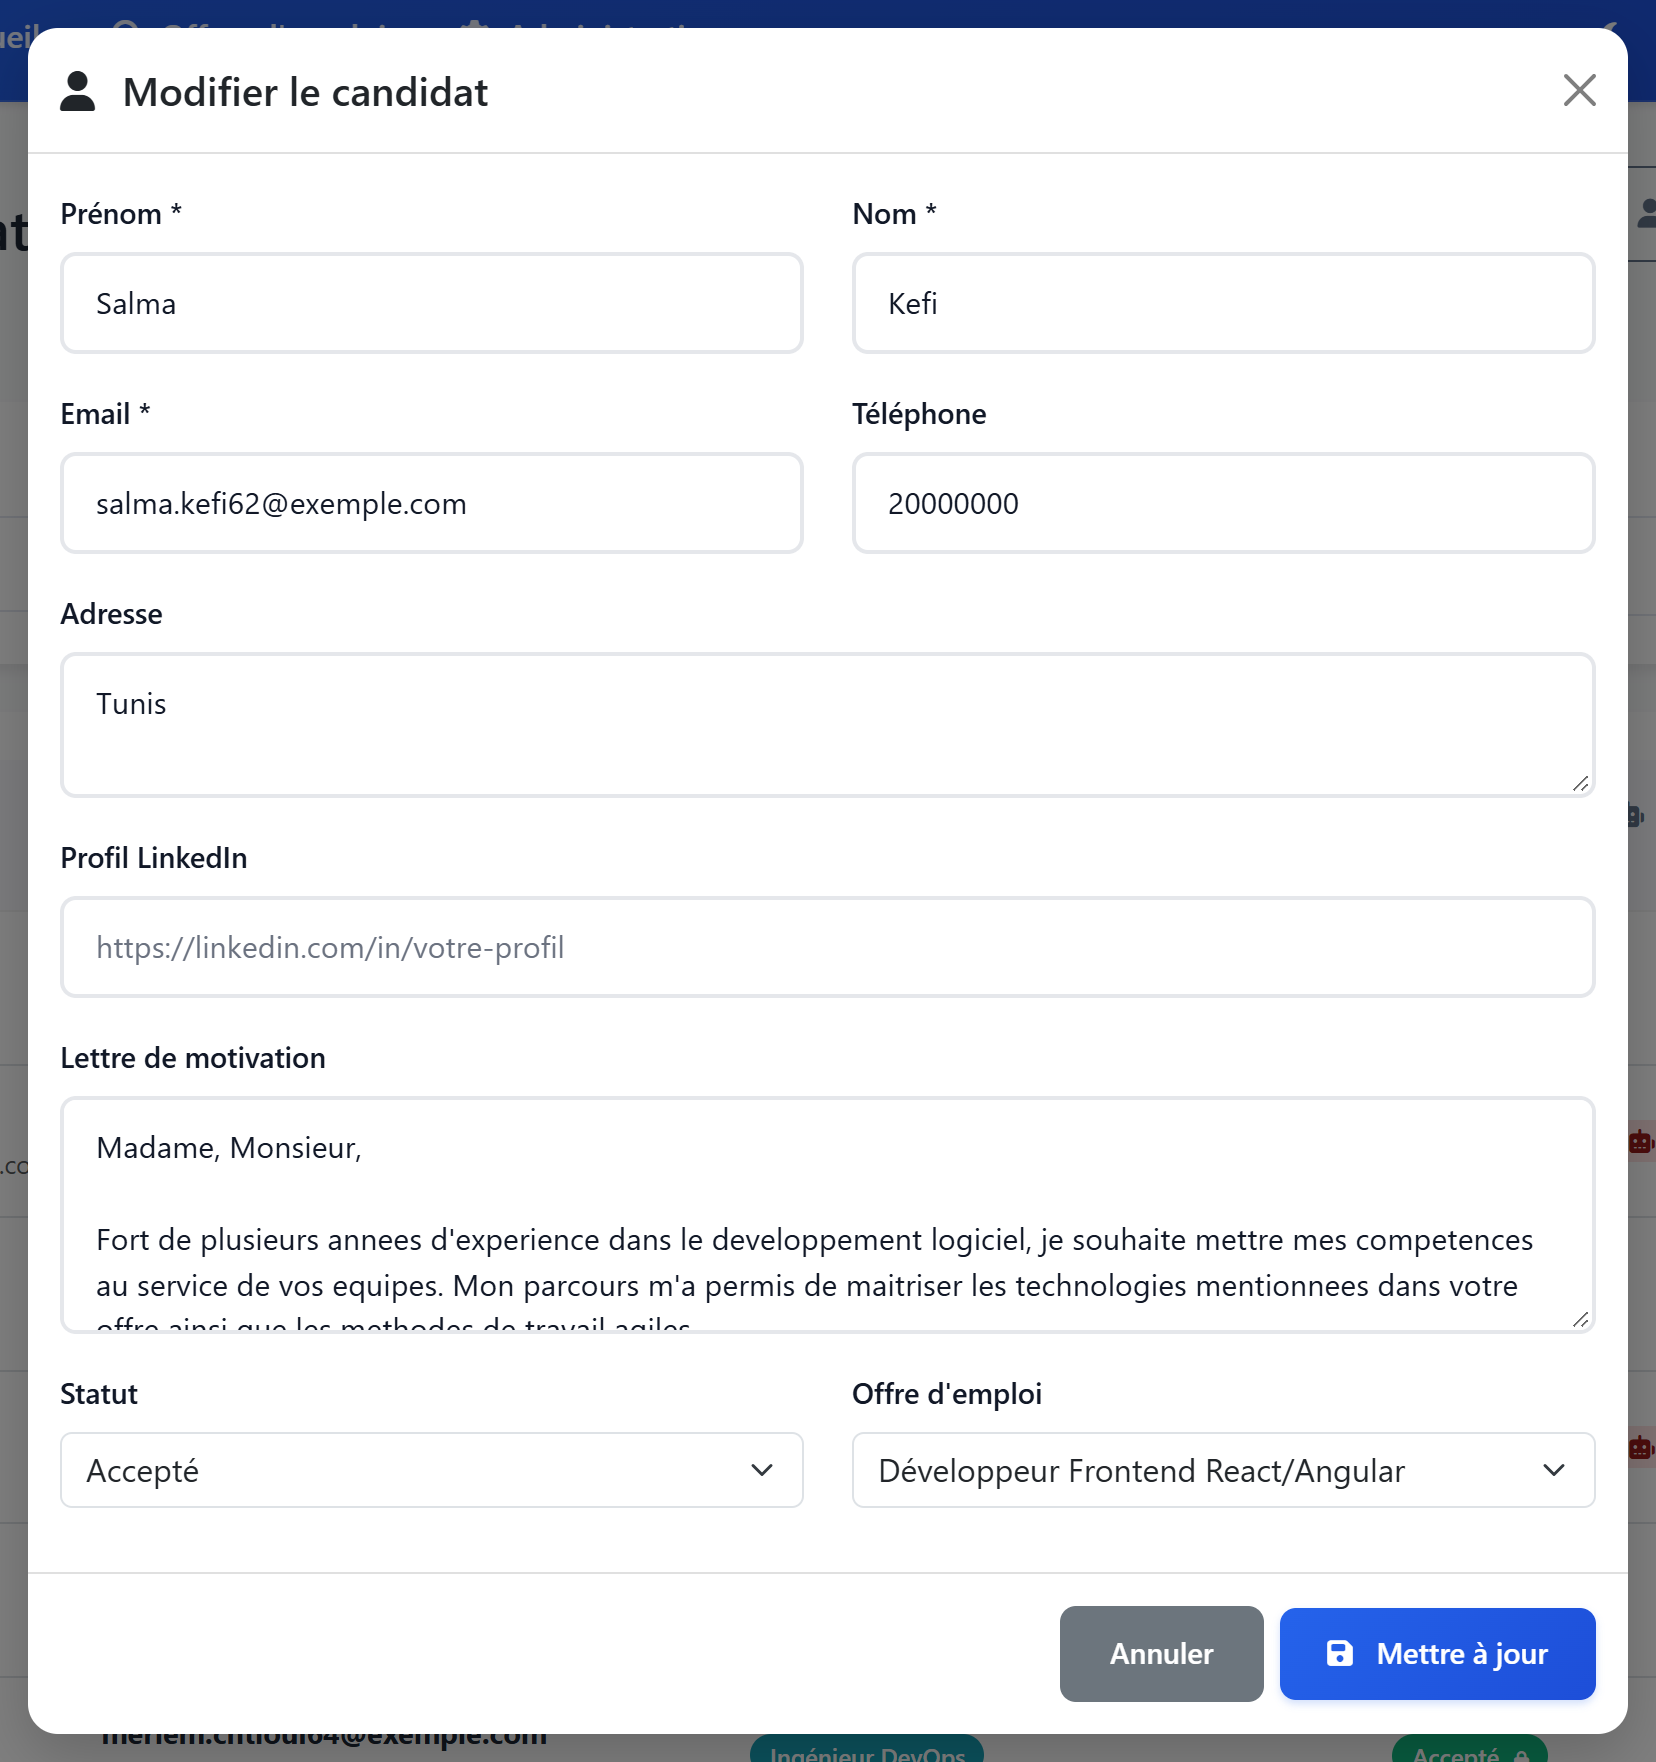
\includegraphics[width=\textwidth, height=0.80\textheight, keepaspectratio]{fig4_9}
\caption{Modification d’un dossier candidat}
\label{fig_4_9}
\end{figure}

Le formulaire de modification (figure~\ref{fig_4_9}) permet de corriger un dossier candidat (coordonnées, lettre, statut, offre associée) ; la fiche de consultation associée regroupe le CV, consultable en ligne sans téléchargement, l’analyse IA détaillée (technique, communication, séniorité) et l’historique des agents n8n sur ce dossier.

% figure 4.10
\setcounter{figure}{9}
\begin{sidewaysfigure}
\centering
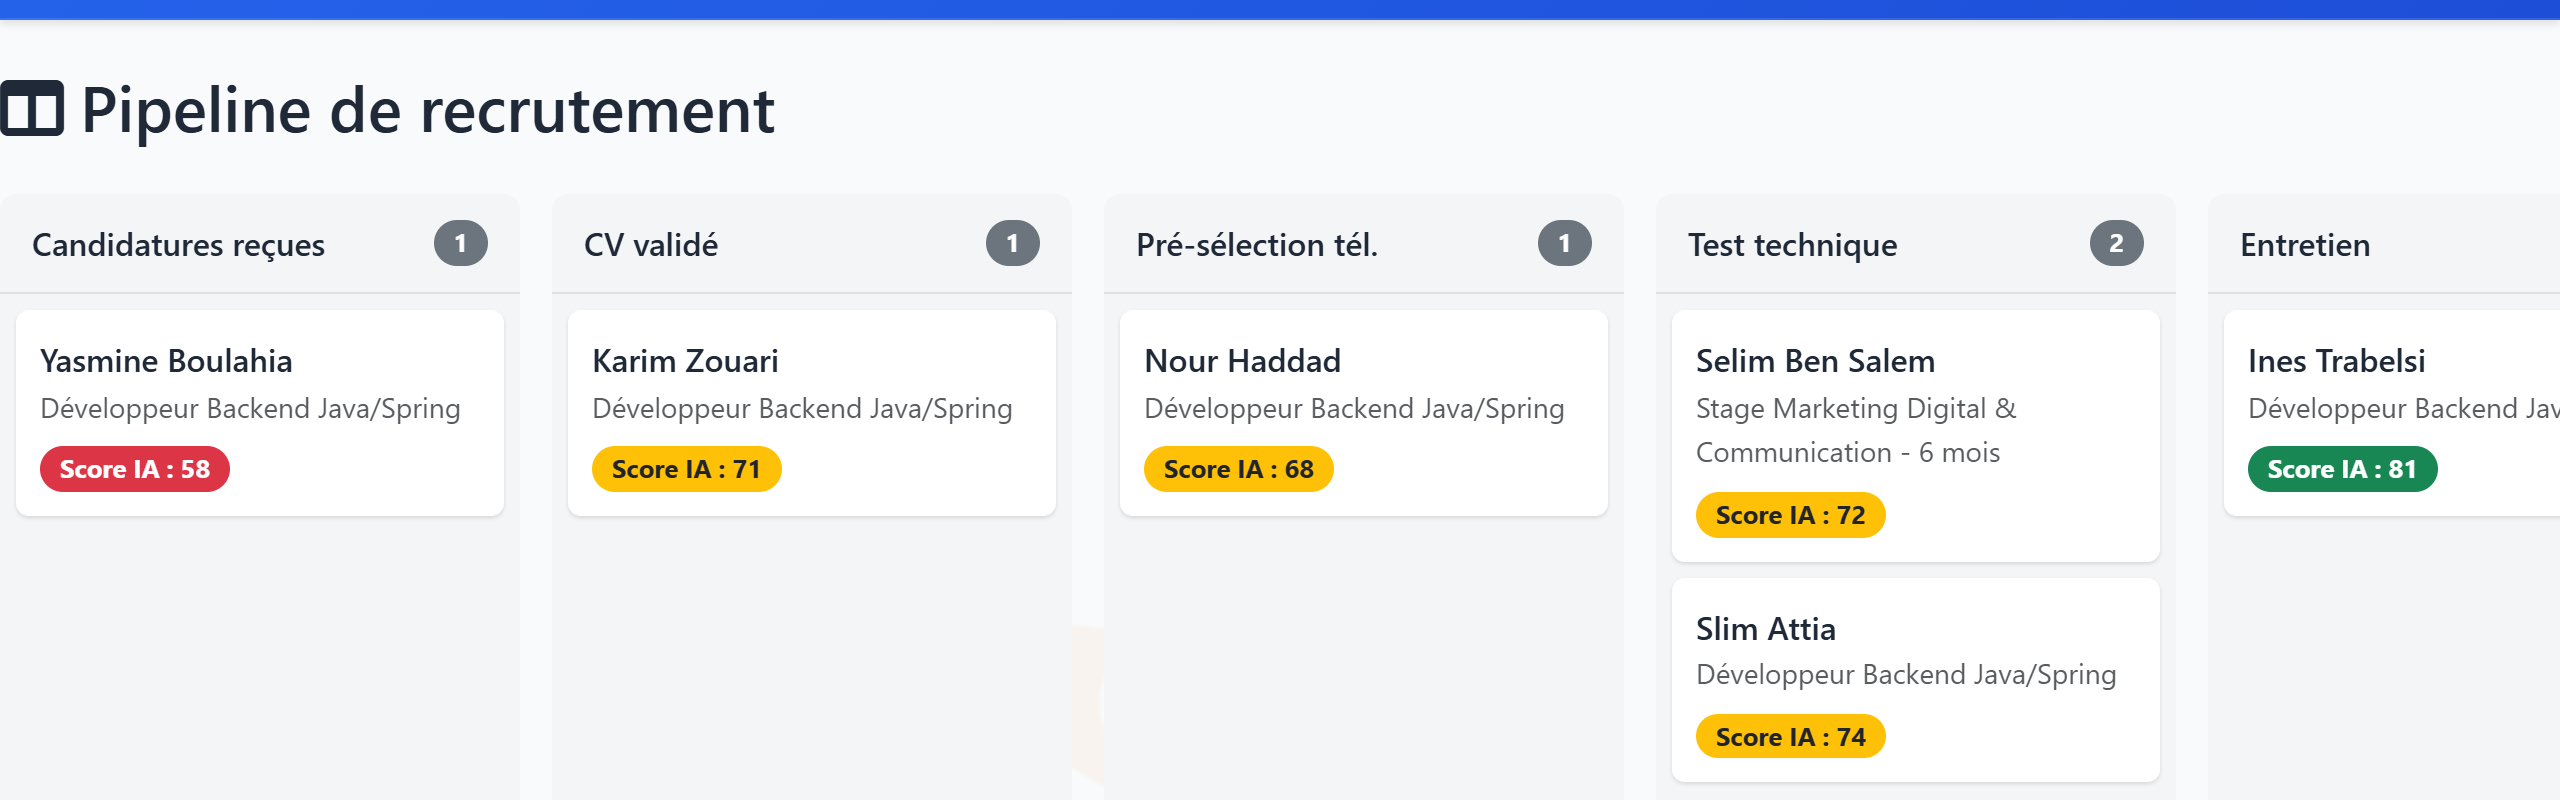
\includegraphics[width=0.98\textheight, height=0.62\textheight, keepaspectratio]{fig4_10}
\caption{Tableau Kanban du pipeline de recrutement}
\label{fig_4_10}
\end{sidewaysfigure}

Le tableau Kanban de la figure~\ref{fig_4_10}, intitulé « Pipeline de recrutement », donne une vue synthétique et interactive de toutes les candidatures réparties par statut : chaque colonne porte le nombre de dossiers qu’elle contient et chaque carte le nom du candidat, l’offre visée et son score IA. Toutes les colonnes ne tenant pas à l’écran, le tableau se fait défiler horizontalement. Glisser une carte d’une colonne à une autre déclenche automatiquement la mise à jour du statut, sous réserve des garde-fous métier décrits au chapitre 3 pour les décisions finales.

% figure 4.11
\setcounter{figure}{10}
\begin{sidewaysfigure}
\centering
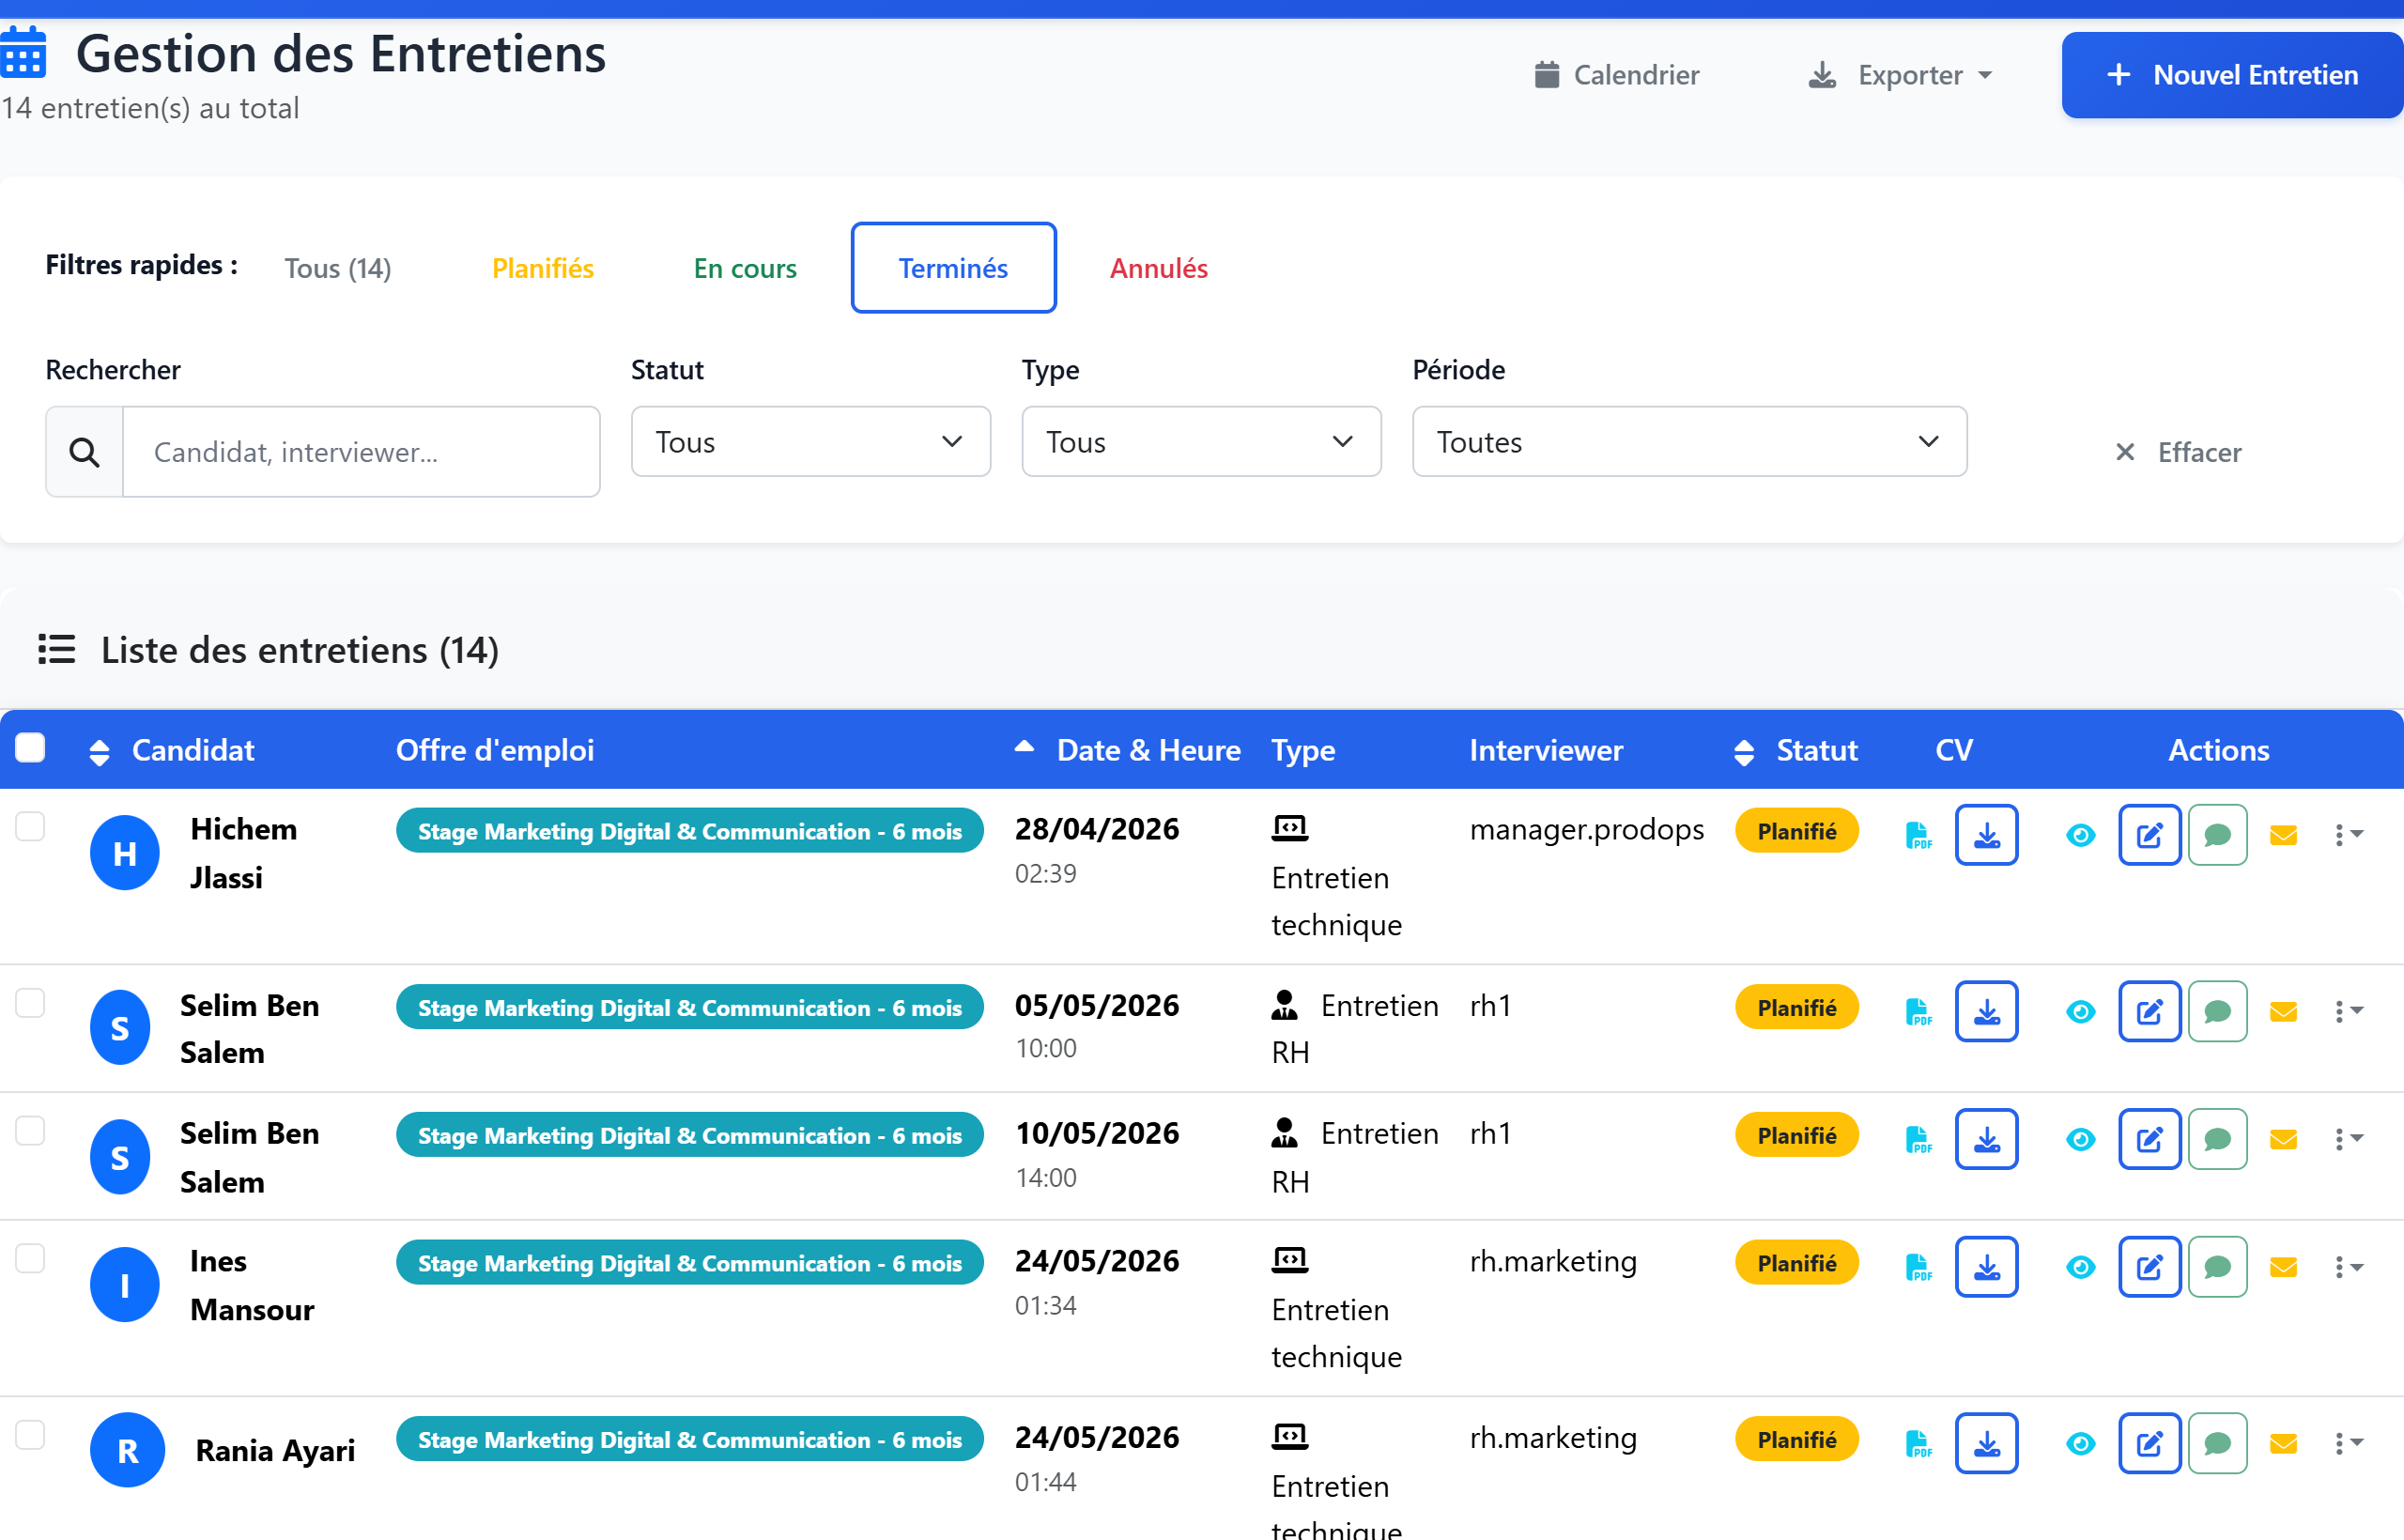
\includegraphics[width=0.98\textheight, height=0.62\textheight, keepaspectratio]{fig4_11}
\caption{Gestion des entretiens (espace RH)}
\label{fig_4_11}
\end{sidewaysfigure}

L’écran de gestion des entretiens de la figure~\ref{fig_4_11} permet de planifier, filtrer et suivre les entretiens par candidat, offre, type, interviewer et statut, avec des actions contextuelles comme le démarrage, l’annulation, la reprogrammation ou l’ajout d’un feedback une fois l’entretien terminé.

% figure 4.12
\setcounter{figure}{11}
\begin{sidewaysfigure}
\centering
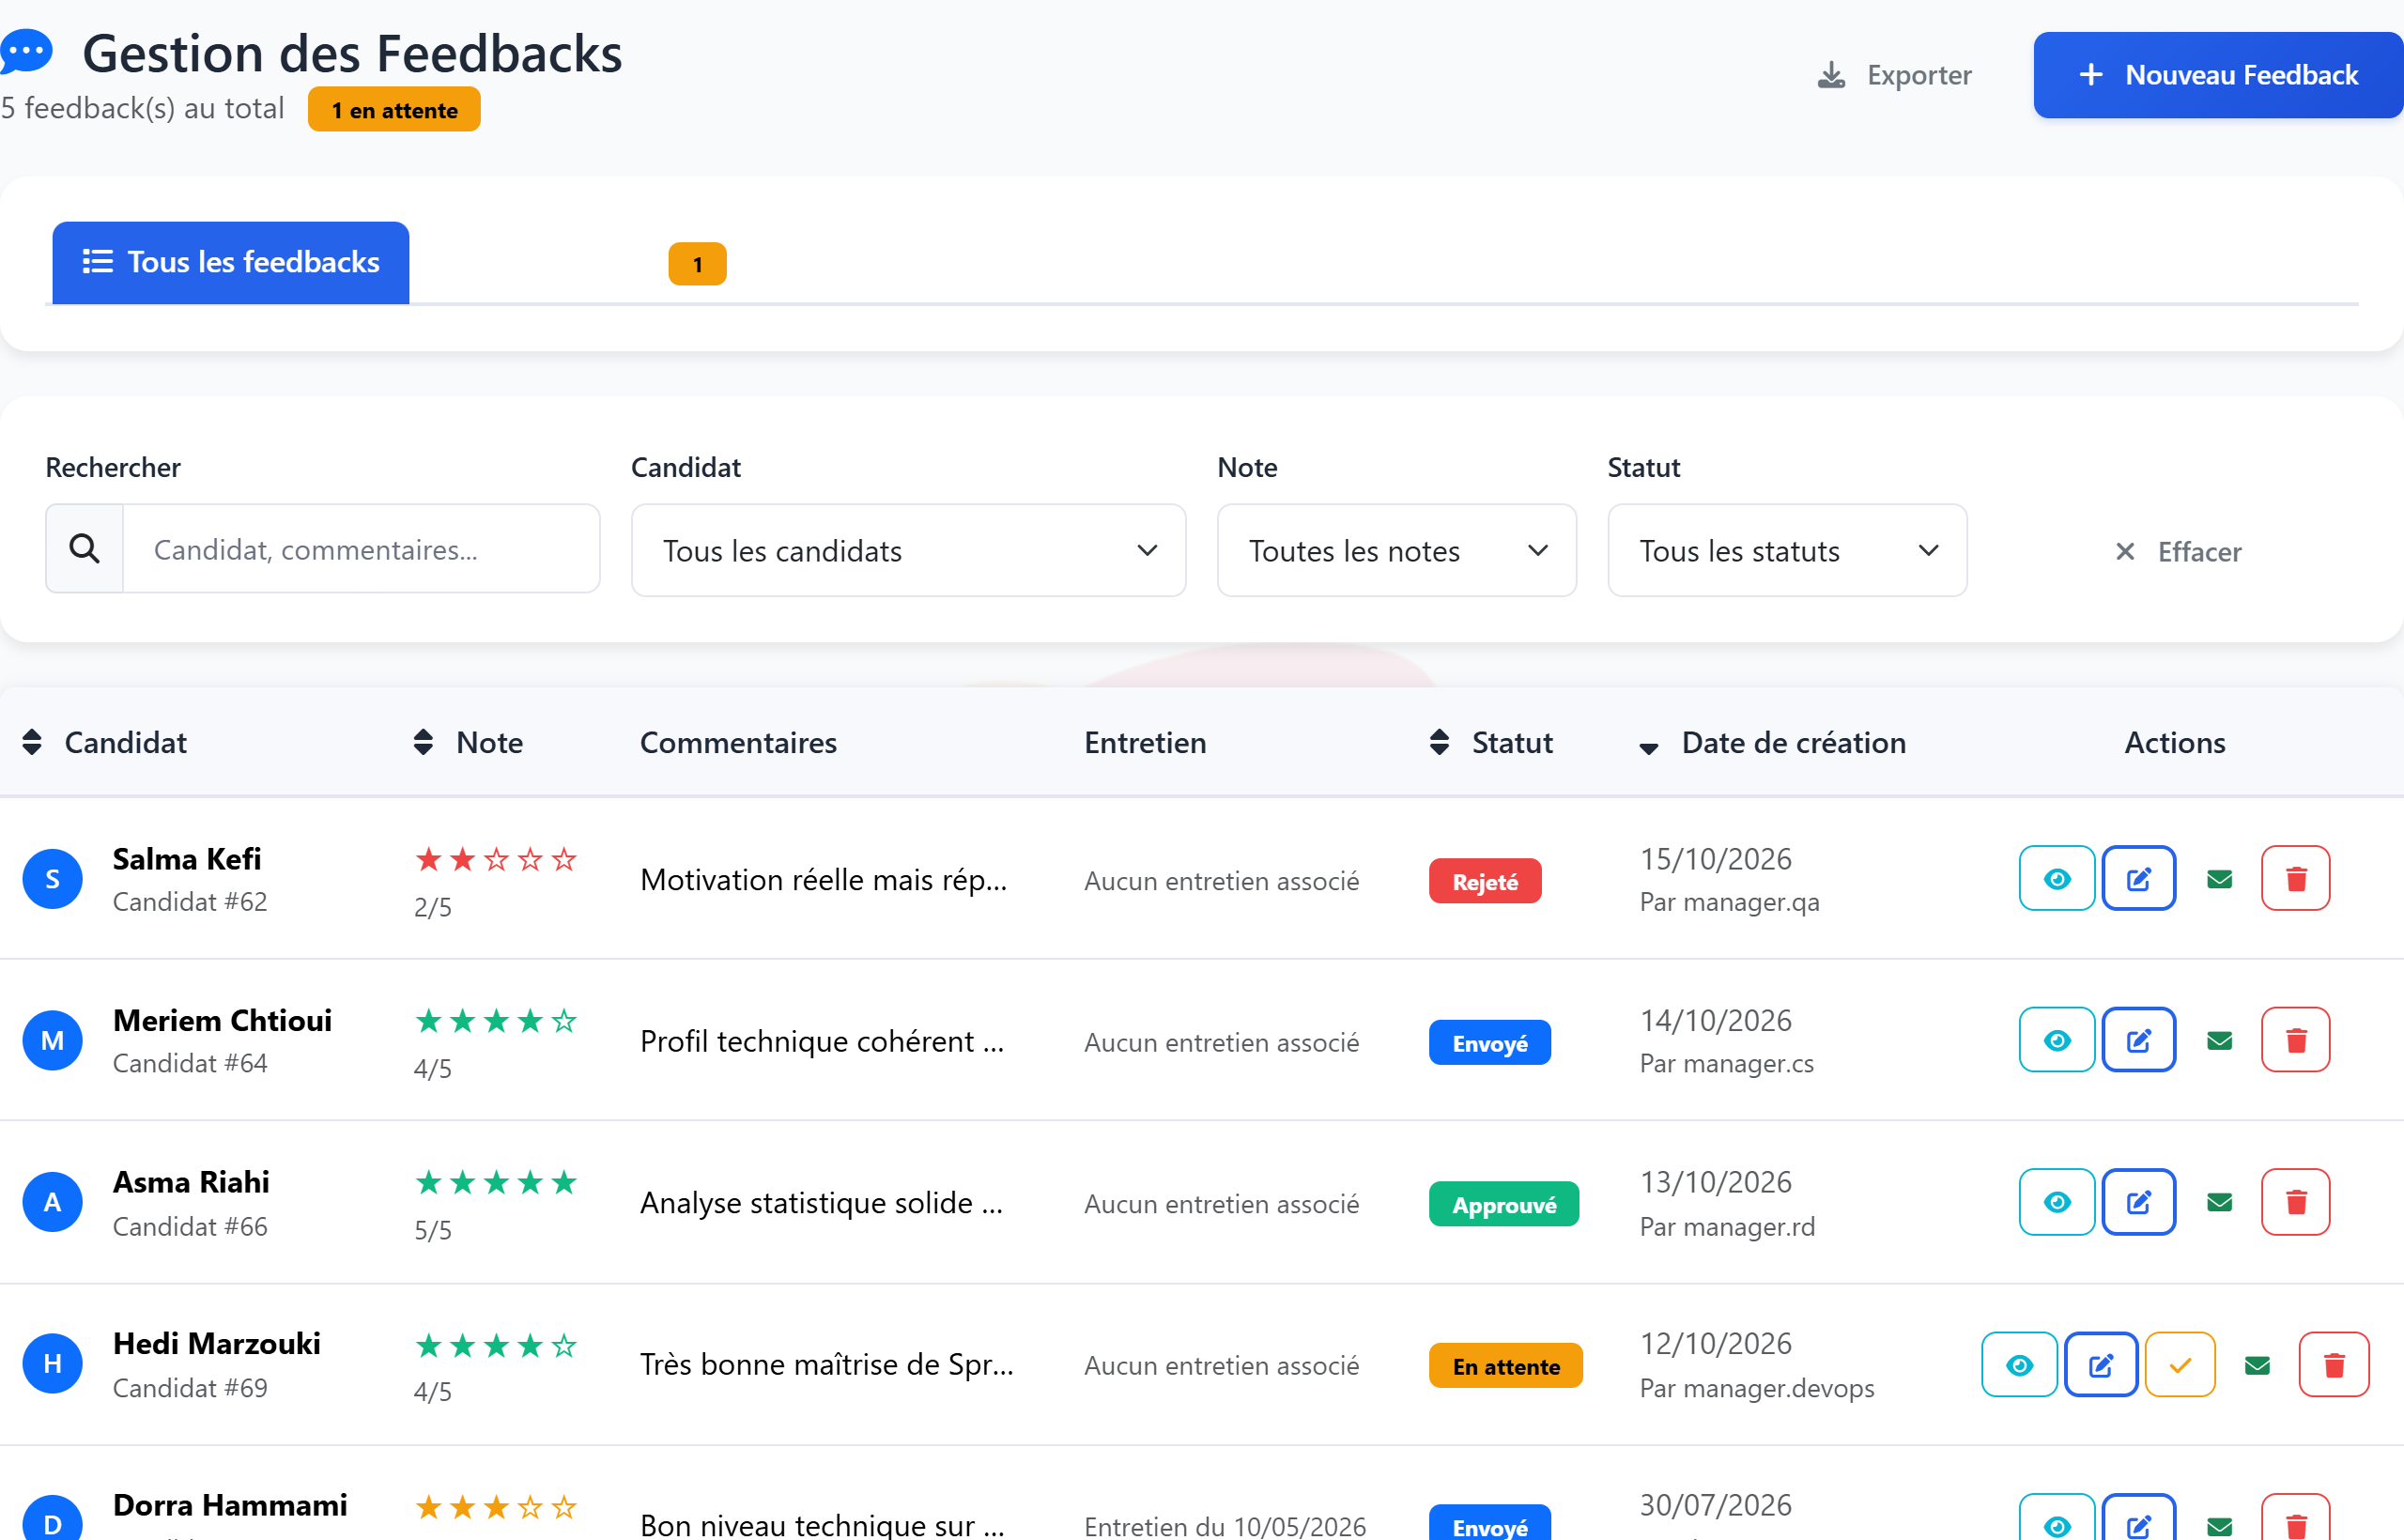
\includegraphics[width=0.98\textheight, height=0.62\textheight, keepaspectratio]{fig4_12}
\caption{Gestion des feedbacks (espace RH)}
\label{fig_4_12}
\end{sidewaysfigure}

La figure~\ref{fig_4_12} centralise les feedbacks saisis par les managers, notés de 1 à 5 étoiles et assortis d’un commentaire, avec une étape de validation par le RH avant transmission au candidat.

% figure 4.13
\setcounter{figure}{12}
\begin{figure}[!ht]
\centering
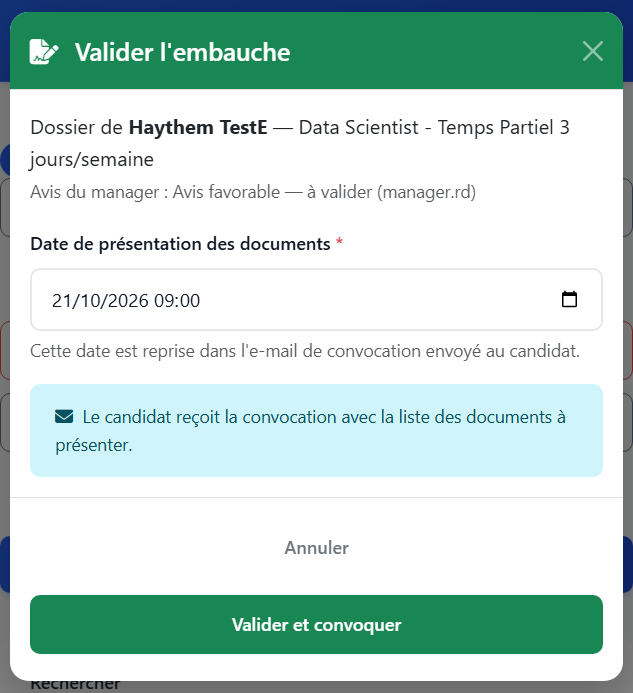
\includegraphics[width=\textwidth, height=0.80\textheight, keepaspectratio]{fig4_13}
\caption{Contreseing RH d’un avis favorable « Valider l’embauche »}
\label{fig_4_13}
\end{figure}

La figure~\ref{fig_4_13} présente la modale dans laquelle le RH contresigne l’avis favorable du manager avant l’embauche ; la date de présentation y est obligatoire, car elle alimente l’e-mail de convocation.

% figure 4.14
\setcounter{figure}{13}
\begin{figure}[!ht]
\centering
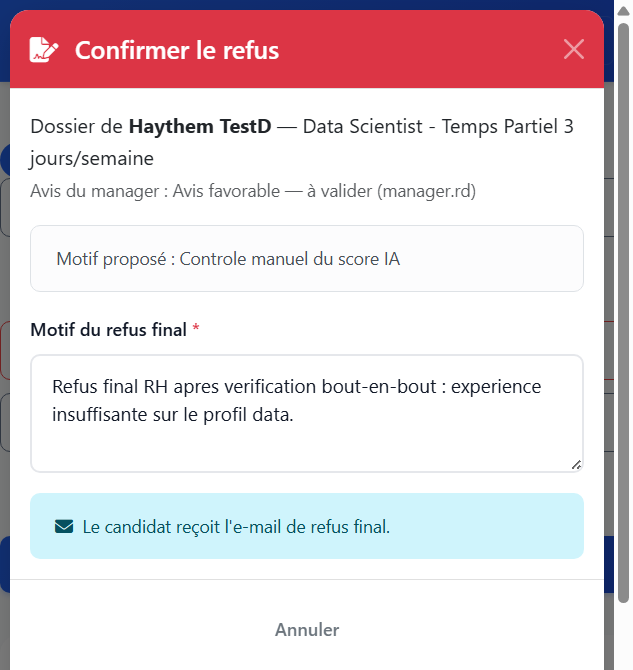
\includegraphics[width=\textwidth, height=0.80\textheight, keepaspectratio]{fig4_14}
\caption{Contreseing RH d’un refus proposé — modale « Confirmer le refus »}
\label{fig_4_14}
\end{figure}

La figure~\ref{fig_4_14} présente la modale « Confirmer le refus », dans laquelle le RH contresigne le refus proposé par le manager. Le motif y est obligatoire, mais il ne part pas dans l’e-mail adressé au candidat — celui-ci ne reprend que le nom du candidat et l’intitulé de l’offre : le motif est la trace humaine de la décision, enregistrée sur le dossier (statusReason) et journalisée dans l’audit.

\subsection{Espace manager}
\label{sec_4_3_3}
% figure 4.15a
\setcounter{figure}{14}
% La capture originale fait 2664 x 1484 px : a cette taille, un texte de 22 px
% n'imprime qu'a 5,9 pt en paysage, ce qui est illisible sur projection comme sur
% papier. Elle est donc recadree en deux volets complementaires, chacun ramene a
% moins de 1760 px de large, soit 8,5 a 9,2 pt imprimes. Le ratio de chaque volet
% (3,0 et 3,0) rend le paysage nettement plus grand que le portrait.
\begingroup\renewcommand{\thefigure}{4.15a}
\begin{sidewaysfigure}
\centering
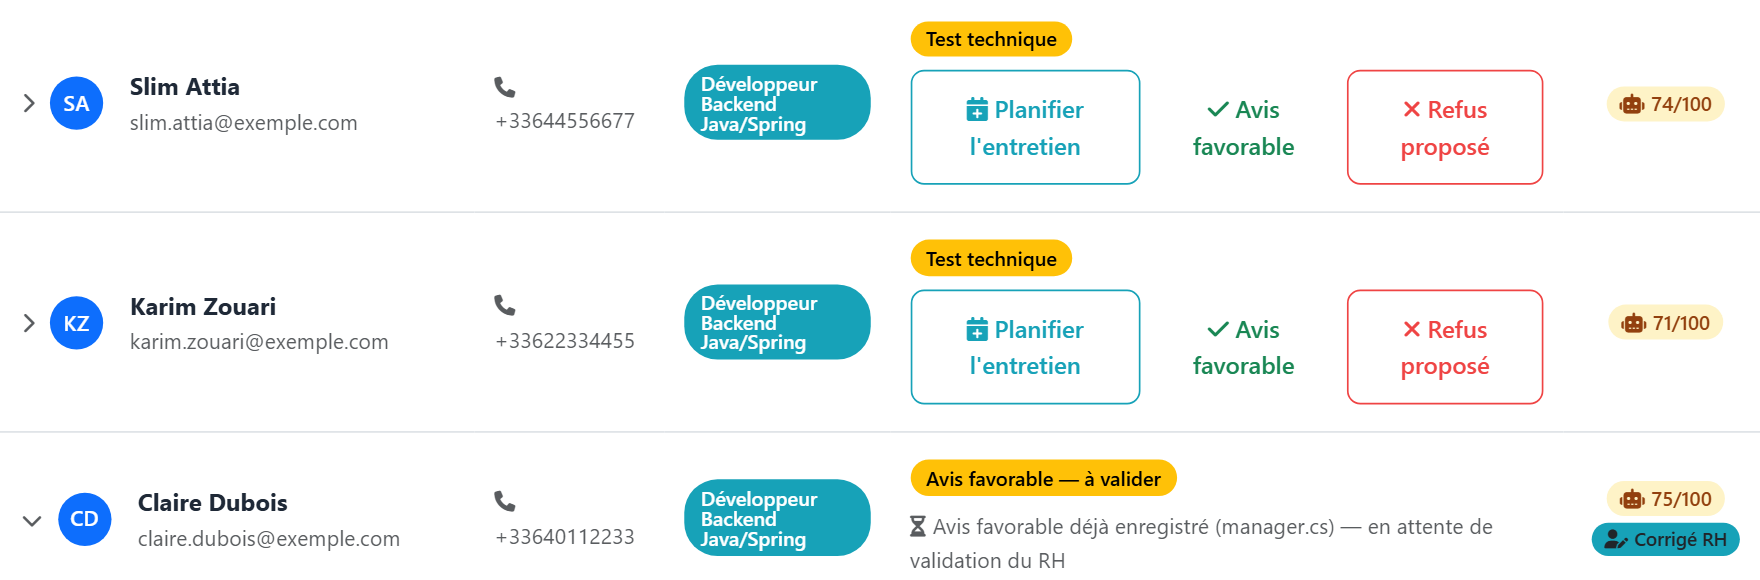
\includegraphics[width=0.98\textheight, height=0.62\textheight, keepaspectratio]{fig4_15a}
\caption{Espace Manager — candidatures du périmètre : état d'avancement, avis du manager et score}
\label{fig_4_15a}
\end{sidewaysfigure}
\endgroup

% figure 4.15b
\setcounter{figure}{14}
\begingroup\renewcommand{\thefigure}{4.15b}
\begin{sidewaysfigure}
\centering
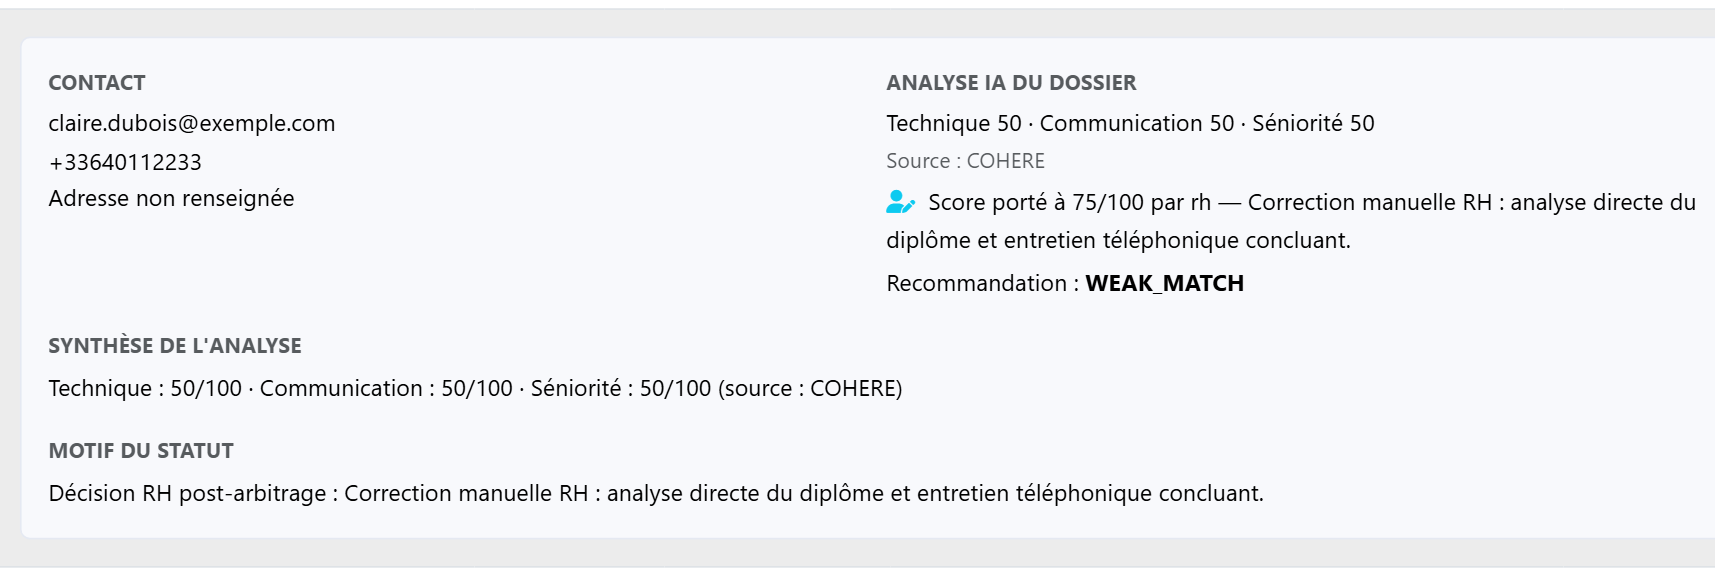
\includegraphics[width=0.98\textheight, height=0.62\textheight, keepaspectratio]{fig4_15b}
\caption{Espace Manager — ligne dépliée : contact, analyse IA du dossier, synthèse et motif du statut}
\label{fig_4_15b}
\end{sidewaysfigure}
\endgroup

Un manager ne voit que les dossiers relevant de son périmètre — le destinataire désigné par le RH, gelé sur la candidature (base MANUAL) et lu par Manager\-Scope\-Service (3.5.4) —, à partir de leur entrée en évaluation technique. La figure~\ref{fig_4_15a} montre cette vue, distincte de la liste RH (figure~\ref{fig_4_7}) : les colonnes ne rognent plus, chaque ligne porte le score et « Planifier l'entretien », et se déplie sur le contact, l'analyse IA du dossier, la synthèse et le motif du statut (figure~\ref{fig_4_15b}). La colonne « Compétences », alignée en regard de l'analyse dans ce panneau, n'y est pas reproduite.

% figure 4.16
\setcounter{figure}{15}
\begin{sidewaysfigure}
\centering
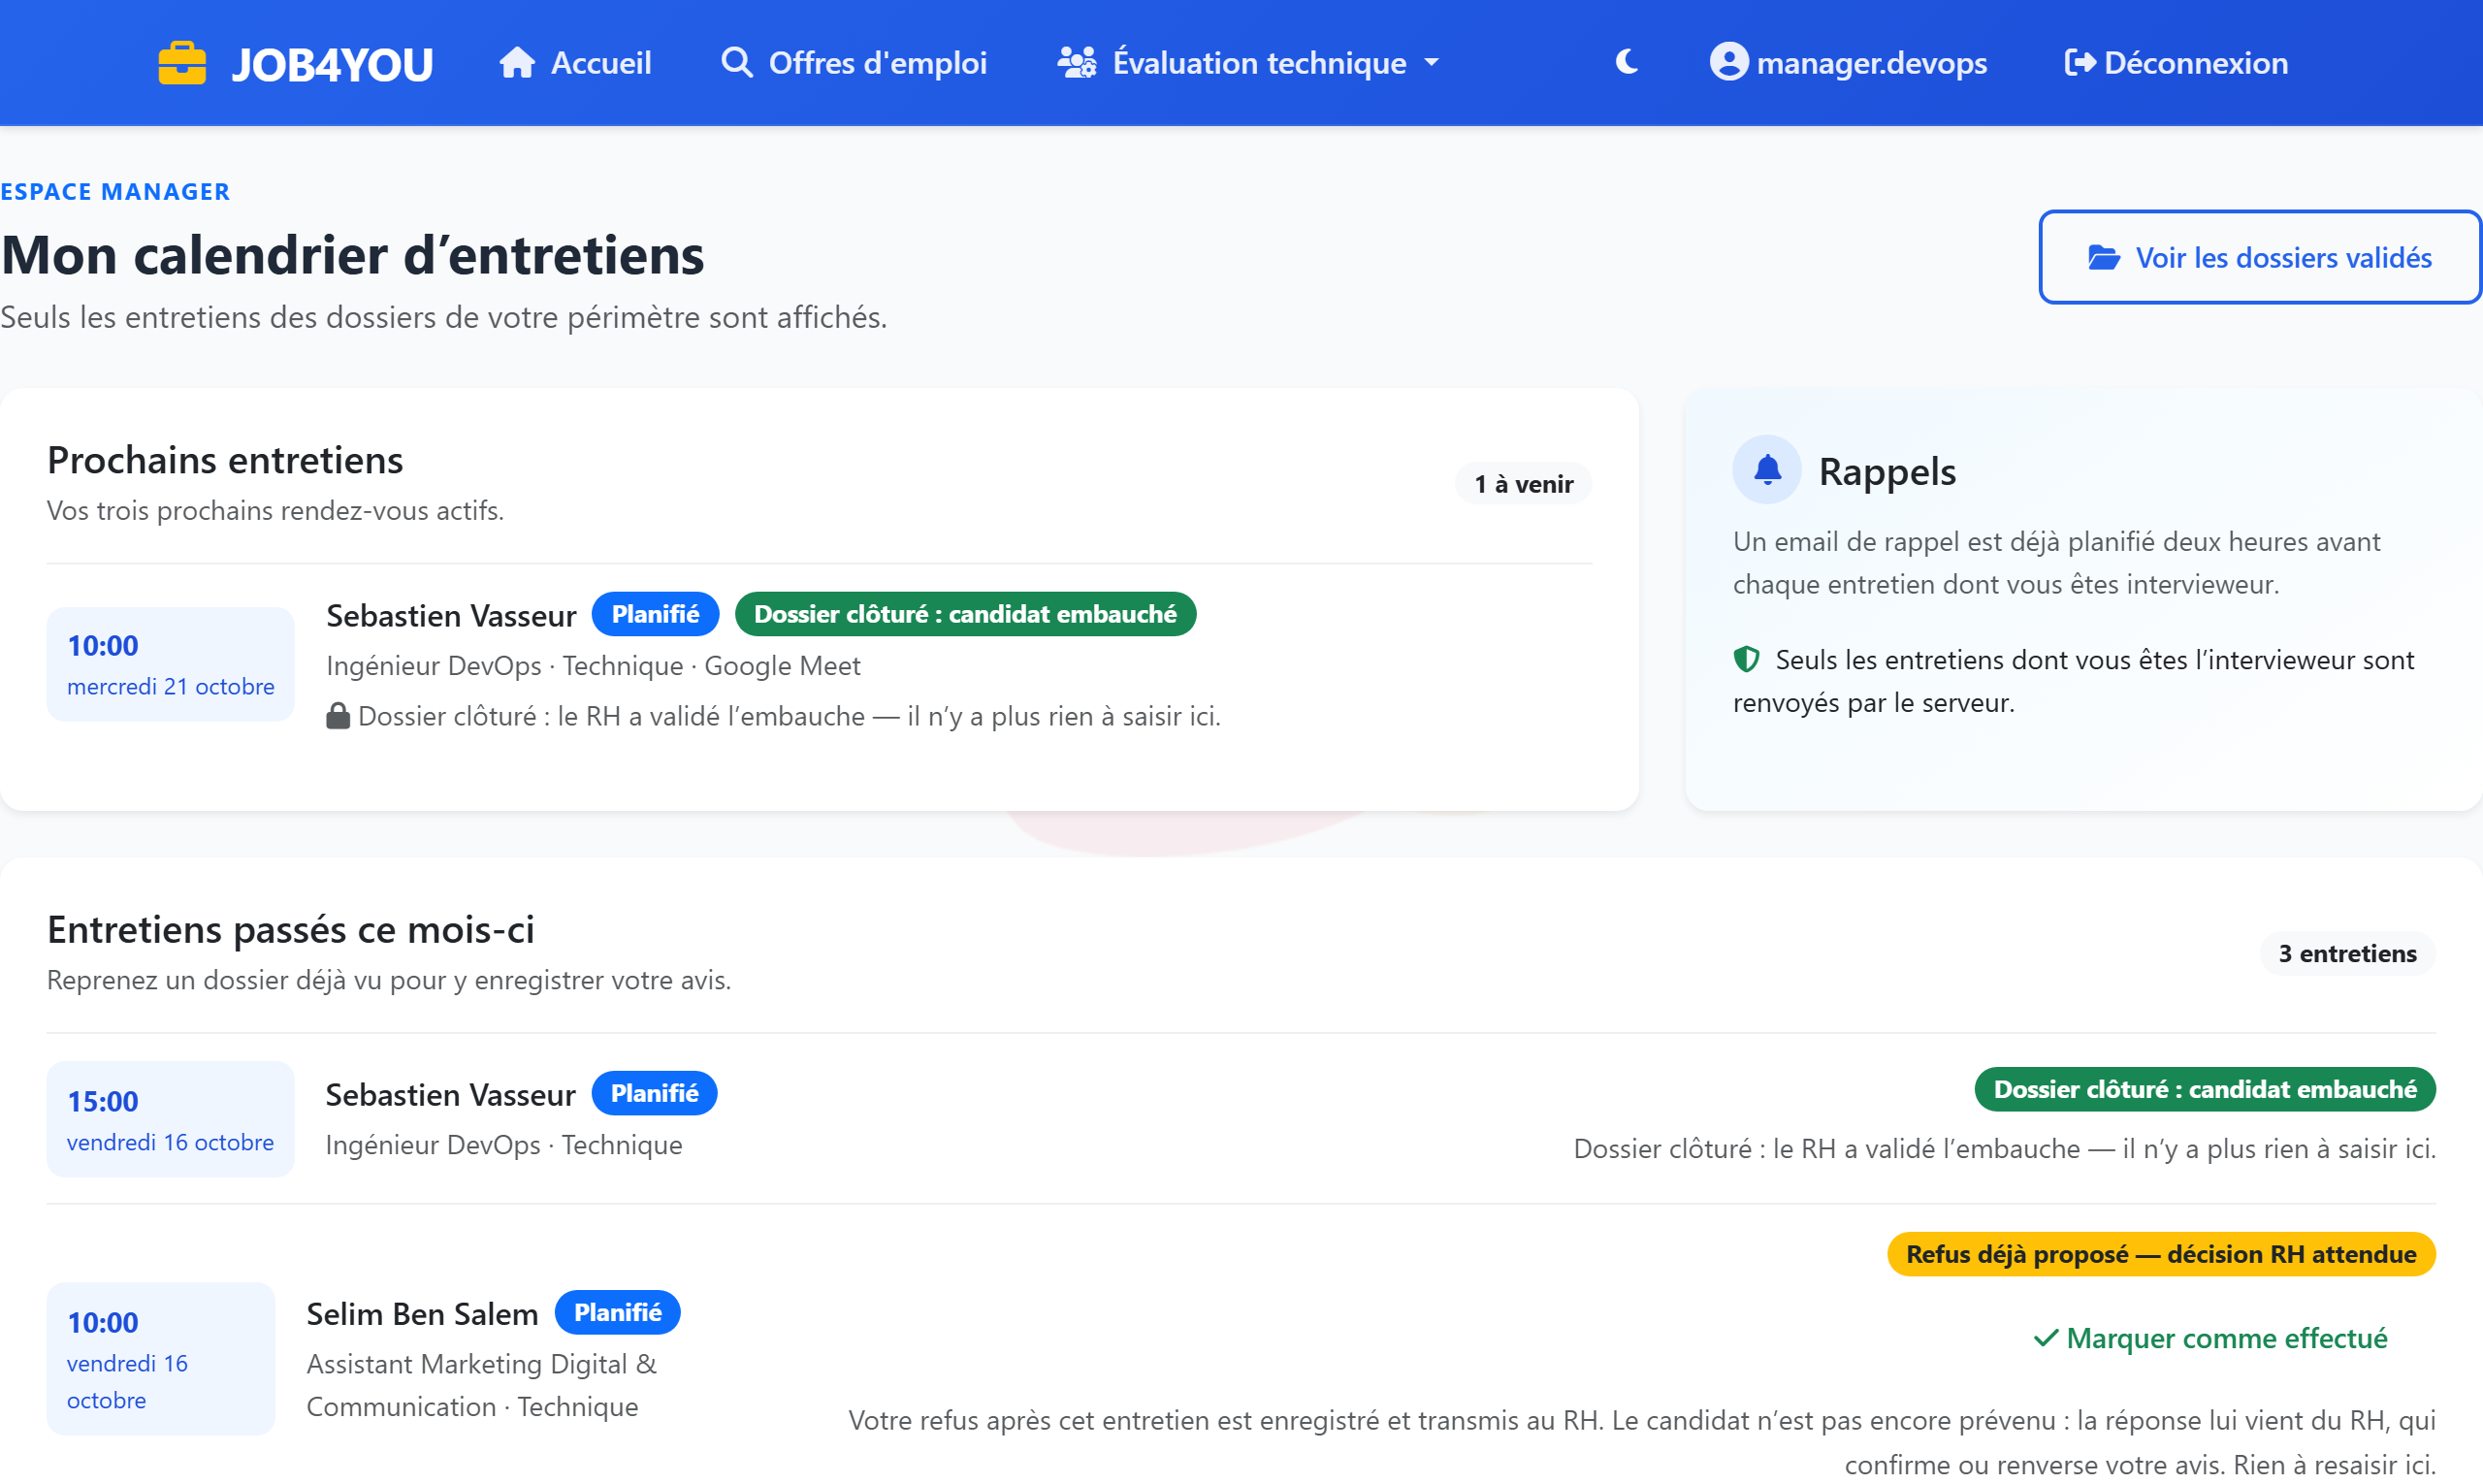
\includegraphics[width=0.98\textheight, height=0.62\textheight, keepaspectratio]{fig4_16}
\caption{Espace Manager — page « Mon calendrier d’entretiens », prochains entretiens, rappels et entretiens passés}
\label{fig_4_16}
\end{sidewaysfigure}

La page « Mon calendrier d’entretiens » (figure~\ref{fig_4_16}) n’affiche que ce qui regarde l’intervieweur connecté : filtrage côté serveur sur sa seule identité, reprise du jeton, et même contrôle d’accès au dossier que pour la liste des dossiers. Elle n’est pas figée pour autant : le manager peut y marquer un entretien comme effectué et y reprendre un dossier encore instruit.

La partie haute de la figure~\ref{fig_4_16} donne les trois prochains rendez-vous actifs, chacun avec l’heure, la date, le candidat, le poste, le format et, une fois le lien produit par l’agent de planification, le bouton « Rejoindre le lien Google Meet » ; l’encart « Rappels » annonce un e-mail deux heures avant chaque entretien dont l’utilisateur est l’intervieweur. La section « Entretiens passés ce mois-ci » permet de reprendre un dossier déjà vu : le manager peut y marquer l’entretien comme effectué et, tant que le dossier est encore en cours d’instruction, l’ouvrir par le bouton « Donner mon avis », qui amène la fiche où l’avis se saisit. Lorsque l’avis a déjà été rendu ou que le dossier est clôturé, ce bouton disparaît et la carte affiche l’état courant (« Dossier clôturé : candidat embauché », « Dossier clôturé : refus validé par le RH »), pour ne jamais laisser le manager devant une commande sans effet. Plus bas, une grille mensuelle — non reproduite ici — complète la page : chaque créneau y est coloré selon l’état du dossier, verrouillé et grisé une fois la décision du RH tombée, ambré et marqué d’un sablier tant que l’avis du manager attend son contreseing. Chaque événement ouvre une fenêtre de détail (candidat, poste, format, date, heure, durée, lieu, notes) où le lien Meet reste derrière un bouton explicite « Rejoindre l’entretien », tant que le créneau court : consulter le planning ne déclenche pas d’appel visio, et l’écran sans lien produit le dit au lieu d’afficher un bouton vide.

\subsection{Administrateur — comptes, paramétrage et traçabilité}
\label{sec_4_3_4}
% figure 4.17
\setcounter{figure}{16}
% Capture recadree sur les trois colonnes utiles (identifiant, e-mail, roles) et
% sur huit lignes : de 2880 x 1560 px a 1720 x 964 px. Un texte de 22 px dans
% l'image passe ainsi de 4,6 pt a 9,2 pt imprimes. Le ratio 1,78 rend le paysage
% nettement plus grand que le portrait (717 pt contre 484), d'ou sidewaysfigure.
\begin{sidewaysfigure}
\centering
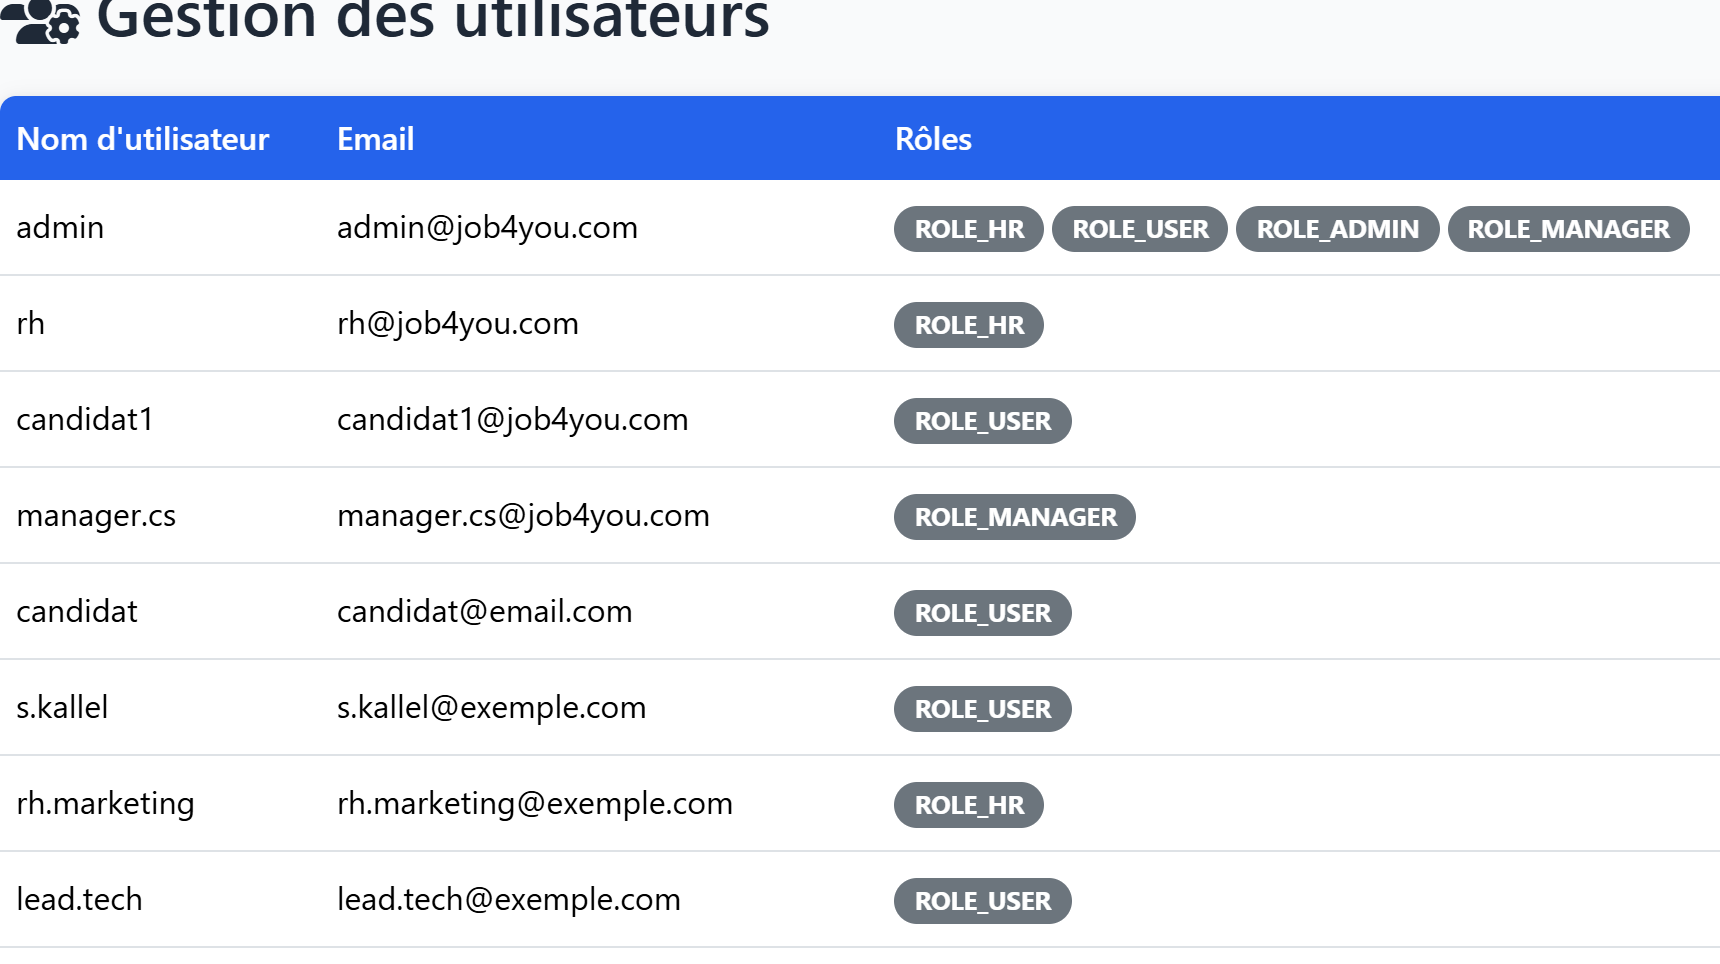
\includegraphics[width=0.98\textheight, height=0.62\textheight, keepaspectratio]{fig4_17}
\caption{Gestion des utilisateurs et des rôles (espace Administrateur) --- partie gauche de l'écran}
\label{fig_4_17}
\end{sidewaysfigure}

L’écran de la figure~\ref{fig_4_17} permet à l’administrateur de gérer l’ensemble des comptes de la plateforme et leurs rôles — un même compte pouvant en cumuler plusieurs —, ainsi que leur rattachement à un département ou, à défaut pour un manager, à une famille de métier.

% figure 4.18
\setcounter{figure}{17}
\begin{sidewaysfigure}
\centering
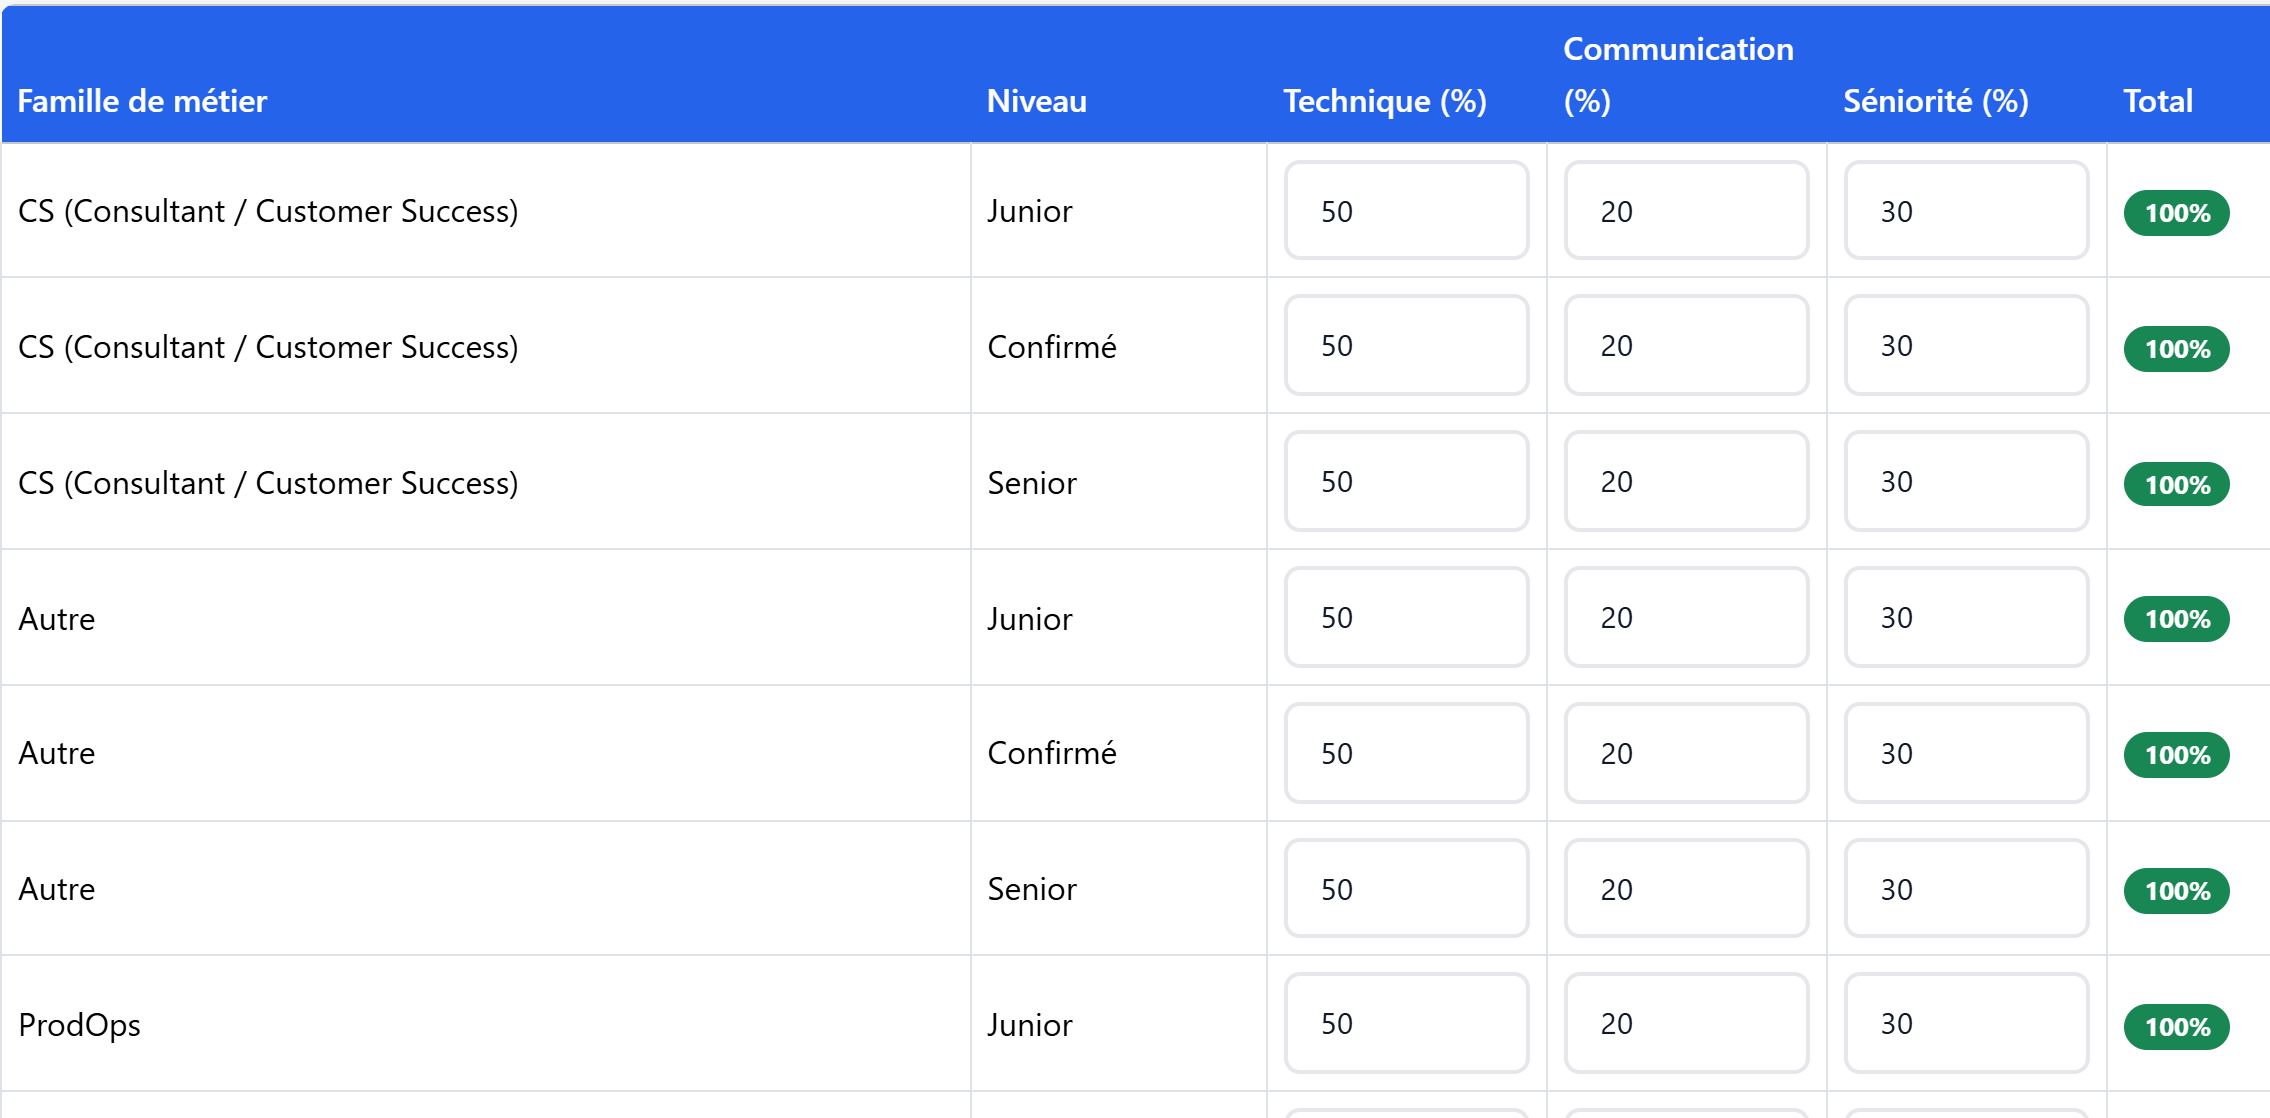
\includegraphics[width=0.98\textheight, height=0.62\textheight, keepaspectratio]{fig4_18}
\caption{Paramétrage du scoring IA par famille de métier}
\label{fig_4_18}
\end{sidewaysfigure}

Réservé à l’administrateur, l’écran de la figure~\ref{fig_4_18} permet d’ajuster, pour chaque famille de métier et chaque niveau de séniorité, la pondération technique / communication / séniorité utilisée par l’agent IA pour calculer le score d’une candidature ; une colonne de contrôle vérifie avant l’enregistrement que les trois poids somment bien à 100 \%.

% figure 4.19
\setcounter{figure}{18}
\begin{sidewaysfigure}
\centering
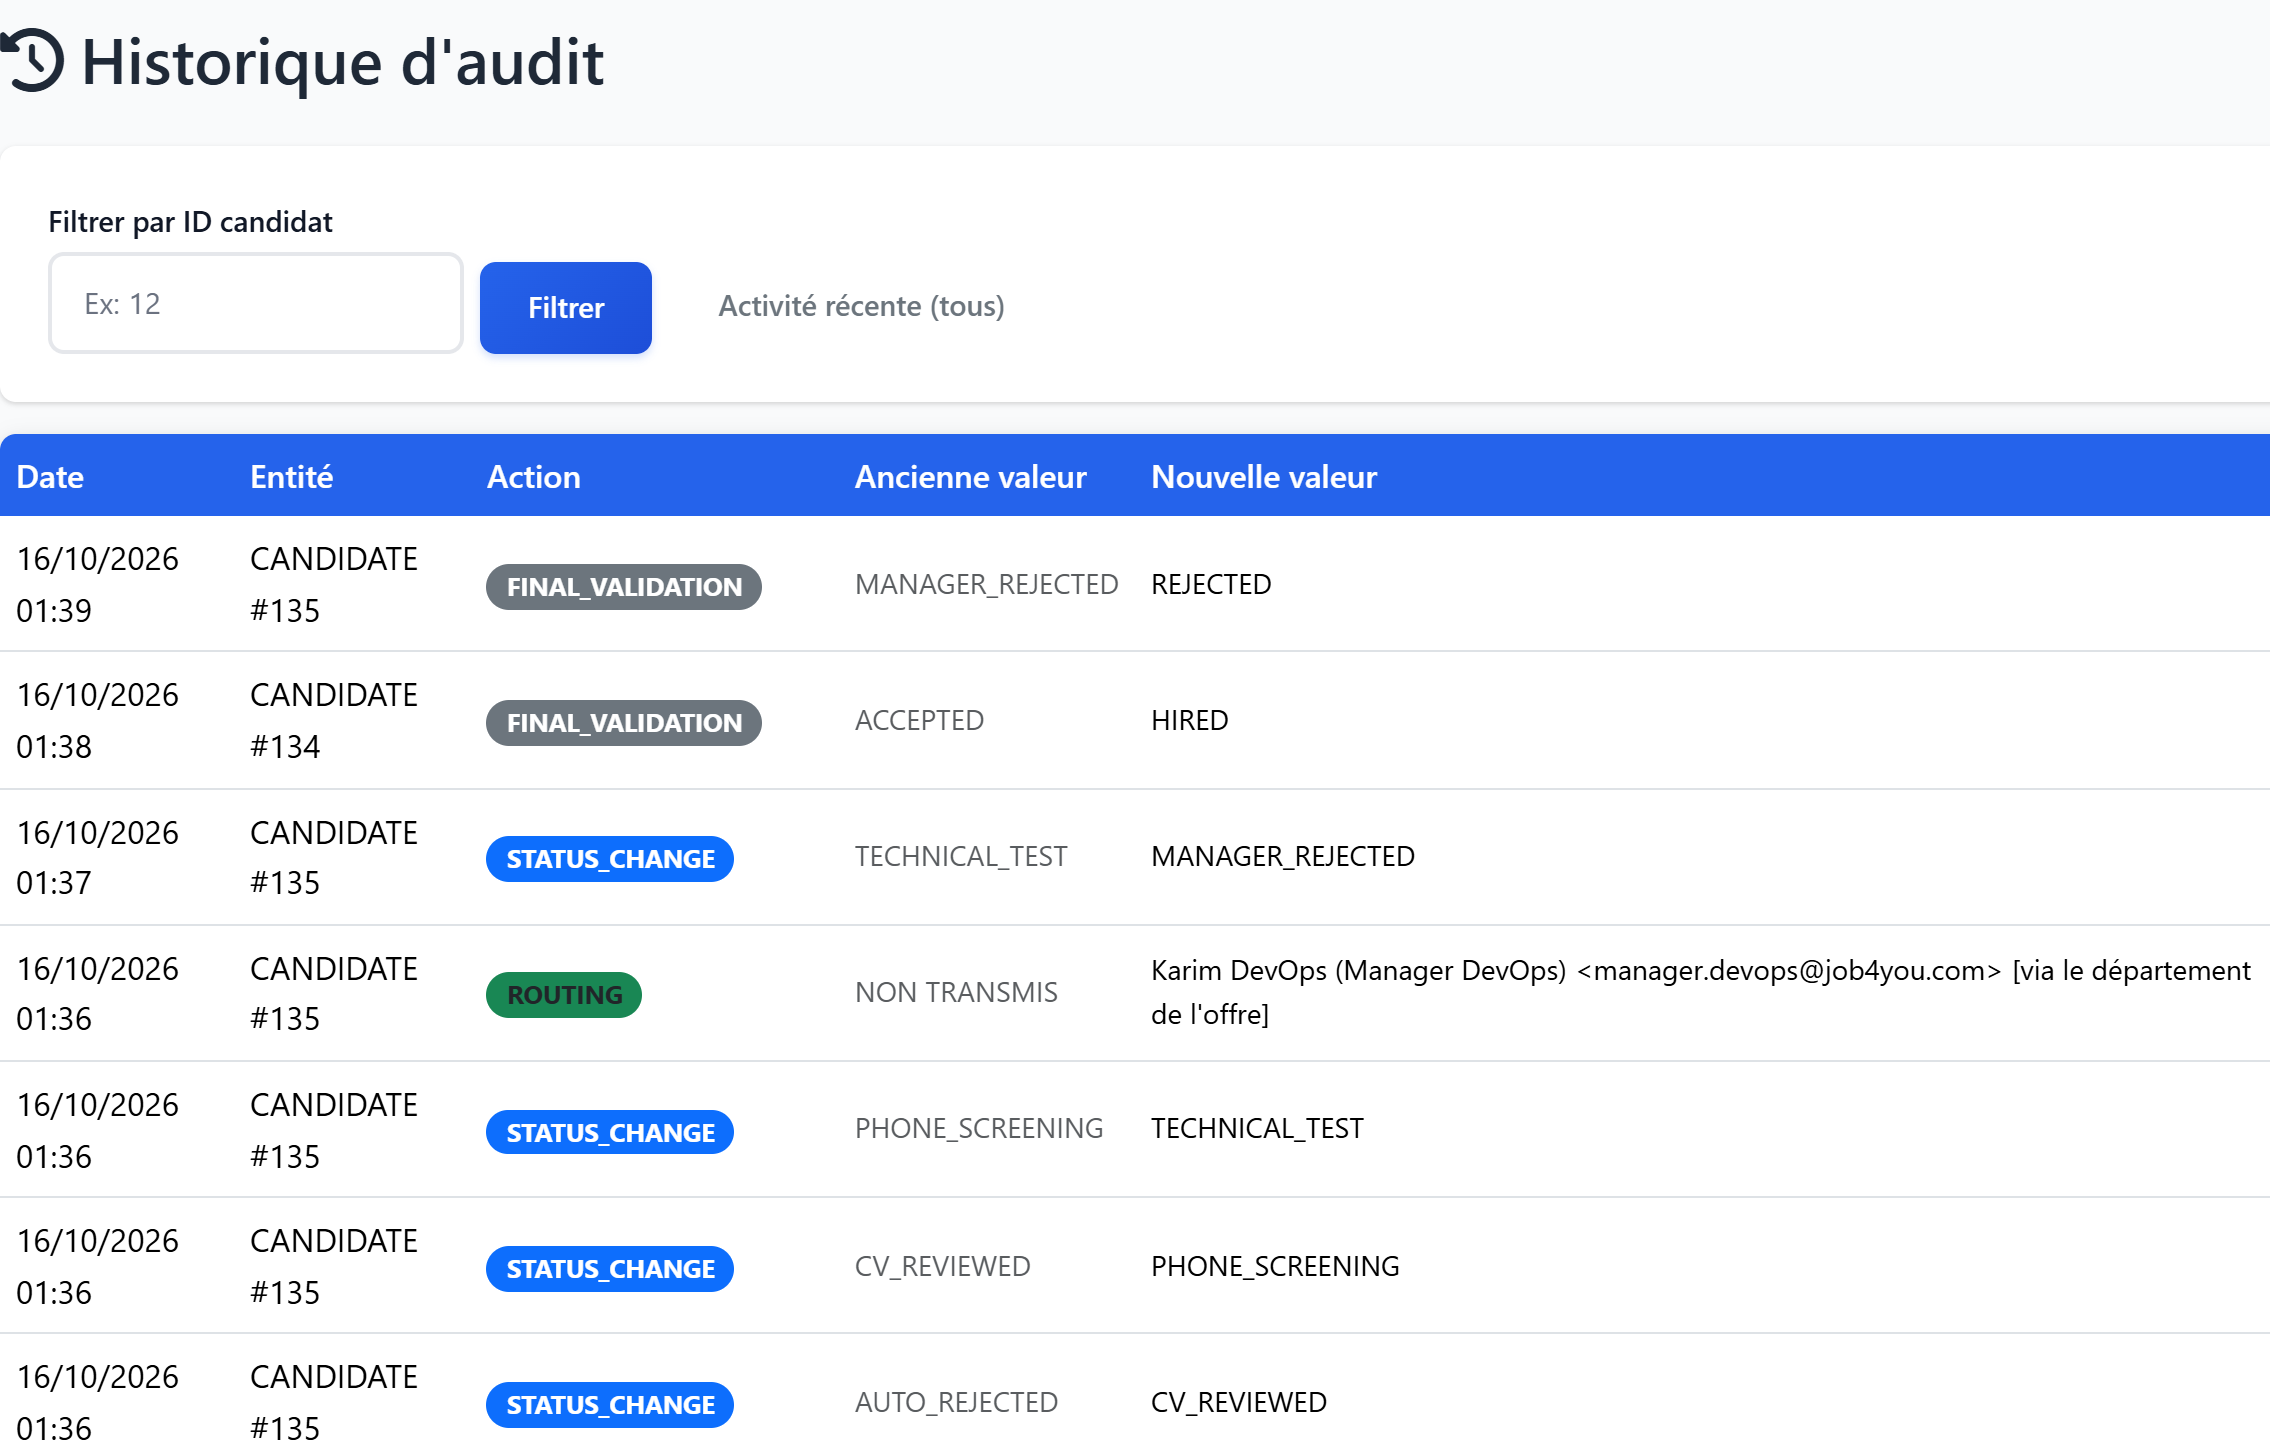
\includegraphics[width=0.98\textheight, height=0.62\textheight, keepaspectratio]{fig4_19}
\caption{Historique d’audit}
\label{fig_4_19}
\end{sidewaysfigure}

L’historique d’audit reproduit en figure~\ref{fig_4_19} trace tous les changements significatifs d’un dossier — statut, score, routage vers un manager, contreseing de la décision finale — en précisant la date, l’entité concernée, la nature de l’action, la valeur précédente et la nouvelle valeur ; une colonne « Effectué par », placée à droite de l’écran et non reproduite sur le recadrage, nomme l’auteur de chaque écriture, qu’elle soit initiée manuellement par un utilisateur ou automatiquement par le système (agents n8n). Les lignes ROUTING et ROUTING\_MANUAL y rappellent le destinataire retenu et la proposition écartée, ce qui garantit la traçabilité de chaque décision.

\subsection{Automatisation n8n et notification du candidat}
\label{sec_4_3_5}
% figure 4.20
\setcounter{figure}{19}
\begin{sidewaysfigure}
\centering
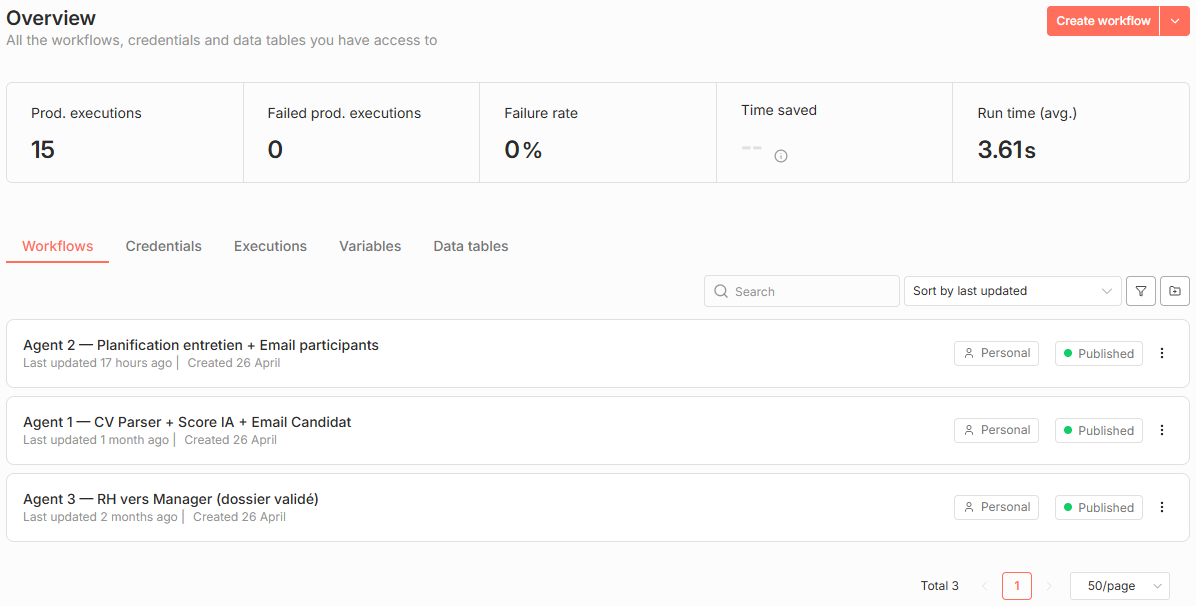
\includegraphics[width=0.98\textheight, height=0.62\textheight, keepaspectratio]{fig4_20}
\caption{Console n8n — les trois flux d’automatisation publiés et leurs statistiques}
\label{fig_4_20}
\end{sidewaysfigure}

Au-delà des interfaces de la plateforme, la chaîne d’automatisation a été vérifiée dans la console n8n elle-même. La figure~\ref{fig_4_20} montre les trois flux déclarés dans l’application — « Agent 1 — CV Parser + Score IA + Email Candidat », « Agent 2 — Planification entretien + Email participants » et « Agent 3 — RH vers Manager (dossier validé) » — tous trois à l’état Publié ; le bandeau de la console affiche 119 exécutions de production, 30 en échec, un taux d’échec de 25,2 \% et une durée moyenne de 4,2 s ; ces compteurs proviennent de l’agrégat interne d’n8n, qui dénombre moins d’exécutions que la table (119 contre 154) mais converge exactement sur les trente échecs. Reprise directement dans la table d’exécutions de l’instance à la date de finalisation du rapport, la mesure de référence porte sur 154 exécutions déclenchées par webhook : 124 abouties et 30 en échec. Ces trente échecs sont tous imputables à Agent 2 et concentrés sur la période de calibration des 15 et 18 octobre (identifiants SMTP Gmail refusés, échec du callback de sauvegarde du lien Meet, accès aux variables d’environnement bloqué dans les nœuds) ; ces trois causes ont été corrigées depuis, et aucune exécution en échec n’est postérieure au 18 octobre. La durée moyenne d’une exécution réussie est alors de 5,6 s, Agent 1 et Agent 3 étant les plus lents (respectivement 6,0 s et 6,2 s, l’analyse Cohere et les envois d’e-mail étant exécutés en série). Ces mesures relèvent d’un environnement local et non d’une exploitation en production ; l’échantillon reste trop limité pour valoir test de charge ou garantie de disponibilité.

% figure 4.21
\setcounter{figure}{20}
\begin{sidewaysfigure}
\centering
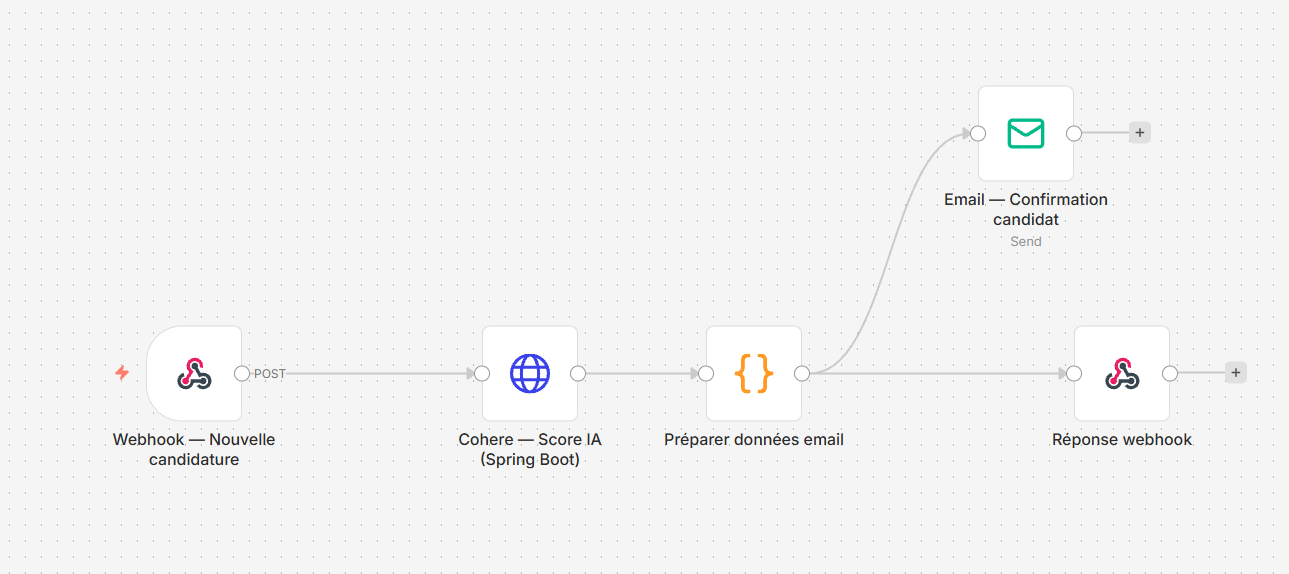
\includegraphics[width=0.98\textheight, height=0.62\textheight, keepaspectratio]{fig4_21}
\caption{Flux n8n de l’Agent 1 — webhook de candidature, appel du scoring Cohere puis e-mail au candidat}
\label{fig_4_21}
\end{sidewaysfigure}

Le détail de l’Agent 1 (figure~\ref{fig_4_21}) confirme le découpage des responsabilités décrit au chapitre 3 : le webhook « Nouvelle candidature » reçoit l’événement POST émis par Spring Boot, le nœud « Cohere — Score IA (Spring Boot) » rappelle le back-end qui interroge réellement l’API de Cohere et persiste le score, puis « Préparer données email » alimente le nœud d’envoi de la confirmation au candidat.

% figure 4.22
\setcounter{figure}{21}
\begin{sidewaysfigure}
\centering
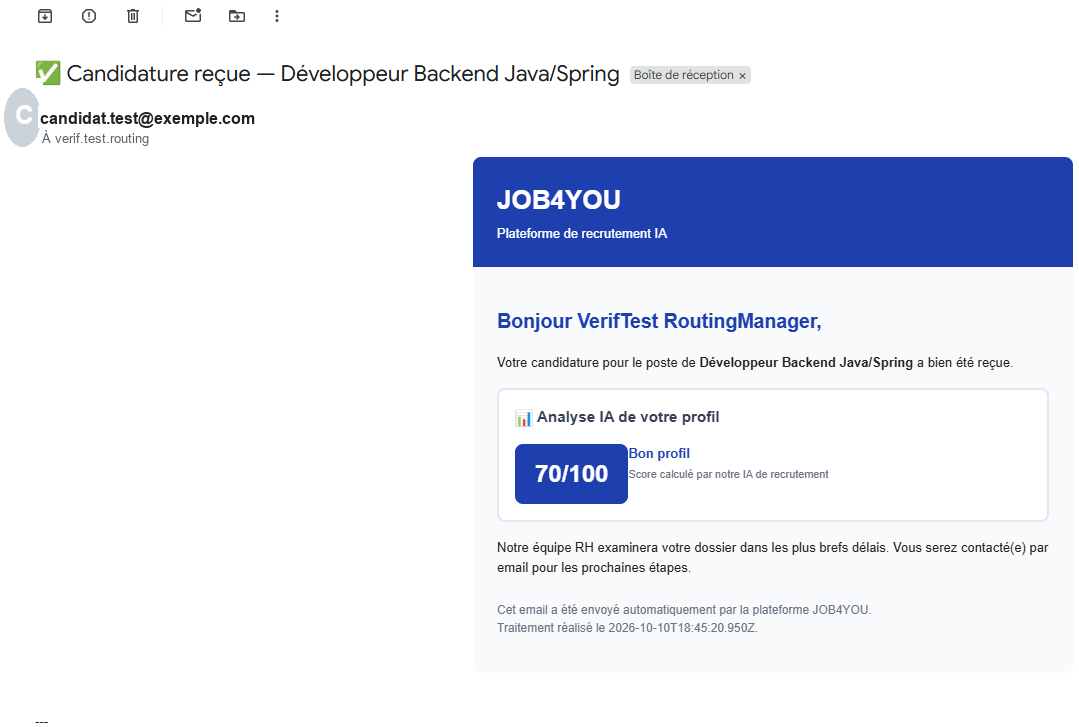
\includegraphics[width=0.98\textheight, height=0.62\textheight, keepaspectratio]{fig4_22}
\caption{E-mail automatique de confirmation de candidature reçu par le candidat}
\label{fig_4_22}
\end{sidewaysfigure}

Côté candidat, la notification produite par ce flux arrive bien dans sa boîte de réception : le corps du message reproduit à la figure~\ref{fig_4_22} est celui généré par l’agent pour une candidature réelle, celle du dossier présenté à la figure~\ref{fig_4_3} — accusé de réception nominatif pour le poste visé, score d’analyse IA obtenu et horodatage du traitement, avec la mention « Cet email a été envoyé automatiquement par la plateforme JOB4YOU ». Lorsque l’analyse n’a pas abouti, le bloc score est remplacé dans le même message par l’encart « profil en cours d’analyse » décrit en section~\ref{sec_4_6}.

\section{Tests}
\label{sec_4_4}
\subsection{Tests unitaires (JUnit 5 / Mockito)}
\label{sec_4_4_1}
Au-delà des vérifications manuelles, la couche service et une partie de la couche controller sont couvertes par une suite de tests automatisés écrite avec JUnit 5 et Mockito \cite{ref16,ref24}, exécutée via Maven. Elle comprend 20 classes de test pour un total de 249 méthodes, toutes exécutées sans échec : Candidate\-Service\-Test, Job\-Offer\-Service\-Test, Manager\-Routing\-Service\-Test, Manager\-Scope\-Service\-Test, Candidate\-Manual\-Routing\-Test, Department\-Proposal\-Service\-Test, N8nServiceTest, N8n\-Service\-Outbox\-Key\-Test, Scoring\-Weight\-Profile\-Service\-Test, Ai\-Scoring\-Service\-Test, Skill\-Normalization\-Service\-Test, Cohere\-Client\-Parsing\-Test, Matching\-Service\-Test, Experience\-Level\-Norms\-Test, Interview\-Service\-Test et Interview\-Service\-Manager\-Calendar\-Test en tests unitaires purs (services isolés à l’aide de doublons Mockito), ainsi que Candidate\-Controller\-Workflow\-Test, Candidate\-Status\-Anonymous\-Security\-Test, Interview\-Manager\-Calendar\-Security\-Test et Interview\-Meet\-Link\-Security\-Test en tests de contrôleur reposant sur @WebMvcTest et MockMvc, qui vérifient les routes anonymes et la sécurité d’accès au lien Google Meet d’un entretien. Ces tests couvrent en particulier la résolution des managers destinataires et son blocage lorsqu’aucun niveau ne propose, le refus de transmission sans désignation et la journalisation ROUTING\_MANUAL d’un choix hors de la proposition retenue, l’isolation stricte de la visibilité à la liste gelée, le calcul du score IA et ses seuils de décision, la neutralisation d’une compétence que le CV nie explicitement, l’orientation de tout score en zone grise vers un arbitrage humain, l’avancée du dossier à l’étape effectivement planifiée, le refus du créneau qui en chevauche un autre à l’agenda du même intervieweur, l’arbitrage RH d’un dossier rejeté par l’agent IA — confirmation motivée ou correction du score —, l’absence de double notification quand le RH confirme un refus déjà notifié par l’IA, ainsi que les garde-fous de transition décrits au chapitre 3.

L’extrait ci-dessous, tiré de Candidate\-Service\-Test, illustre l’un des deux tests ajoutés pour valider le correctif décrit en section~\ref{sec_4_5_4} : il vérifie qu’un manager n’obtient, via get\-Candidates\-By\-Status(), que les candidats de son propre périmètre.

%% extrait reel de Candidate\-Service\-Test.java (lines 861-881)
\begin{lstlisting}[style=CodePFE]
@Test
@DisplayName("getCandidatesByStatus() ne renvoie à un manager que les candidats de son périmètre")
void shouldScopeGetCandidatesByStatusToCurrentManager() {
    Department rd = new Department("R&D", "R&D");
    rd.setId(1L);
    Department devops = new Department("4YOU", "4YOU");
    devops.setId(2L);

    Candidate inScope = candidateWithOffer(60L, "manager.rd@company.com", rd);
    Candidate outOfScope = candidateWithOffer(61L, "manager.devops@company.com", devops);
    User manager = makeManagerUser("manager_rd", "manager.rd@company.com", rd);

    authenticateAs("manager_rd", Role.ERole.ROLE_MANAGER);
    when(userRepository.findByUsername("manager_rd")).thenReturn(Optional.of(manager));
    when(candidateRepository.findByStatus(CandidateStatus.CV_REVIEWED))
            .thenReturn(List.of(inScope, outOfScope));

    List<CandidateResponse> result =
            candidateService.getCandidatesByStatus(CandidateStatus.CV_REVIEWED);

    assertThat(result).extracting("id").containsExactly(60L);
}
\end{lstlisting}

\subsection{Tests fonctionnels manuels}
\label{sec_4_4_2}
Chaque fonctionnalité développée a fait l’objet d’un test fonctionnel manuel directement dans l’application, couvrant à la fois le scénario nominal et les principaux cas d’erreur. Le tableau suivant synthétise les cas de test exécutés et leur résultat.

% tableau 4.1
\setcounter{table}{0}
{\captionsetup{labelsep=colon}
\renewcommand{\arraystretch}{1.25}\footnotesize
\begingroup%
\setlength{\tabcolsep}{4pt}%
\begin{longtable}{|P{0.302\textwidth}|P{0.540\textwidth}|P{0.104\textwidth}|}
\caption{Synthèse des tests fonctionnels réalisés}\label{tab_4_1}\\ \hline
\textbf{Cas de test} & \textbf{Résultat attendu} & \textbf{Résultat obtenu} \\
\hline
\endfirsthead
\multicolumn{3}{l}{\itshape Suite du tableau \ref{tab_4_1}}\\ \hline
\textbf{Cas de test} & \textbf{Résultat attendu} & \textbf{Résultat obtenu} \\
\hline
\endhead
\hline\endfoot
\hline\endlastfoot
Connexion avec identifiants valides & Connexion réussie, jeton JWT renvoyé & OK \\
Connexion avec mot de passe invalide & Erreur 401, accès refusé & OK \\
Accès à une route RH avec un compte Candidat & Erreur 403 (Forbidden) & OK \\
Publication d’une offre d’emploi par le RH & Offre créée et visible sur la page publique & OK \\
Dépôt d’une candidature avec CV & Candidature créée (statut APPLIED), CV stocké et lié au dossier & OK \\
Analyse automatique du CV par l’agent IA & Score calculé, statut CV\_REVIEWED ou AUTO\_REJECTED selon le seuil & OK \\
Avis manager sur un dossier non encore validé par le RH & Erreur 400, avis bloqué par le garde-fou métier & OK \\
Avis manager après validation RH & Avis enregistré (ACCEPTED ou MANAGER\_REJECTED) et notifié au RH, sans e-mail au candidat & OK \\
Planification d’un entretien sur un dossier clos (rejeté/retiré) & Erreur 400, planification bloquée & OK \\
Notification par e-mail au candidat après la décision finale contresignée par le RH & E-mail reçu, contenu cohérent avec le statut & OK \\
Transmission RH $\rightarrow$ manager : l’aiguillage propose, le RH désigne le destinataire & Sans désignation : 400, dossier immobile ; le manager choisi est seul notifié ; choix hors proposition : ROUTING\_MANUAL & OK \\
Notification du manager à l’entrée en Test technique (après entretien téléphonique) & Le manager désigné est notifié à ce stade, pas avant & OK \\
Visibilité d’un manager sur un dossier d’un autre département & Aucun dossier hors de la liste gelée des destinataires n’est visible & OK \\
Retrait d’une candidature (statut WITHDRAWN) & Le dossier quitte la liste active sans rechargement et reste filtrable & OK \\
Acceptation directe d’un candidat depuis CV\_REVIEWED (sans entretien tél.) & Erreur 400, transition refusée & OK \\
Chevauchement de deux entretiens d’un même intervieweur & Erreur 400 ; le même jour reste possible & OK \\
Question du chatbot sur le statut réel d’une candidature & Réponse conforme aux données réelles en base, sans invention & OK \\
Demande du score IA ou de l’identité de l’intervieweur au chatbot & Refus poli, aucune donnée interne révélée & OK \\
Tentative d’injection de prompt sur le chatbot (« ignore tes instructions... ») & Le contexte système n’est pas divulgué, le rôle de l’assistant est conservé & OK \\
Appel du point d’entrée du chatbot sans jeton JWT & Erreur 401, accès refusé & OK \\
Avis manager puis contreseing RH (HIRED avec date / REJECTED motivé) & E-mail de convocation ou de refus motivé au candidat ; erreur 400 si la date ou le motif manque & OK, vérifié le 14/10 en local \\
Transmission aux deux managers d’un dossier et relance d’un envoi échoué & Deux événements distincts, un par destinataire ; la relance émet une nouvelle clé et non un second silence & OK, vérifié le 14/10 en local \\
Arbitrage RH d’un dossier rejeté automatiquement par l’agent IA & Confirmation du refus (REJECTED motivé, sans second e-mail au candidat) ou correction du score (retour en CV\_REVIEWED) ; erreur 400 si le motif manque & OK, vérifié le 17/10 en local \\
\end{longtable}
\endgroup%
}
Ce tableau atteste de l’exécution des vingt-trois scénarios listés, tous concluants ; il ne constitue pas pour autant une garantie globale de qualité. Des cas nominaux et des cas d’erreur qui réussissent ne prouvent ni l’absence de défauts sur les chemins non exercés, ni le comportement de la plateforme sous charge. Ces tests vérifient des fonctionnalités et des règles d’accès : la pertinence du scoring IA, elle, est mesurée en section~\ref{sec_4_4_5}. Aucun test de charge n’a mesuré les exigences de temps de réponse fixées en section~\ref{sec_2_2_3} (moins de 500 ms en lecture, moins de 2 s en écriture), qui restent à valider en préproduction.

\subsection{Tests des API avec Postman et Swagger}
\label{sec_4_4_3}
J’ai testé isolément, à l’aide de Postman, l’ensemble des points d’entrée de l’API REST — en particulier les scénarios d’authentification, de contrôle d’accès par rôle et de gestion des erreurs (404, 400, 403). La documentation interactive Swagger, générée automatiquement à partir des annotations du code, m’a permis de vérifier la cohérence des contrats d’interface tout au long du développement.

\subsection{Vérification de bout en bout}
\label{sec_4_4_4}
Au-delà des tests unitaires par fonctionnalité, j’ai mené une vérification de bout en bout du parcours complet de recrutement : soumission d’une candidature, analyse automatique par l’IA, validation par le RH, planification d’un entretien, saisie d’un feedback, avis du manager puis contreseing du RH — chaque étape déclenchant la notification par e-mail attendue, au candidat et aux parties prenantes internes. Une vidéo de démonstration commentée de ce parcours, courriels remis à l’appui, a été transmise à l’encadrant. Le fractionnement de la décision en deux niveaux, et les erreurs renvoyées quand un manager tente de trancher seul, sont figés par des tests côté back-end (Candidate\-Service\-Test, section~\ref{sec_4_4_1}).

\subsection{Évaluation du matching sur un jeu de référence annoté (Gold Set)}
\label{sec_4_4_5}
Les tests décrits ci-dessus vérifient que la plateforme fonctionne ; ils ne disent rien de la pertinence du score attribué par l’IA. J’ai donc constitué un jeu de référence — un Gold Set \cite{ref21} — de vingt curriculum vitæ synthétiques, rédigés pour ce projet à partir de profils réalistes mais fictifs : aucun CV réel d’un collaborateur de Sopra HR n’a été employé, ce qui écarte toute question de confidentialité dans la démarche d’évaluation.

Les vingt profils se répartissent sur les trois familles de métiers visées par la plateforme, chacune rattachée à une offre cible : Développeur Backend Java/Spring (offre 115, sept profils), DevOps Engineer (offre 117, six profils) et Business Analyst (offre 122, sept profils). Chaque CV porte une vérité terrain binaire, PERTINENT ou NON\_PERTINENT, arrêtée sur des critères objectifs — compétences techniques indispensables et séniorité — et non d’après la sortie du modèle : onze profils sont pertinents, neuf sont volontairement hors cible (compétences d’un autre domaine, séniorité insuffisante, outillage sans rapport avec l’offre). Quatre cas (GOLD\_17 à GOLD\_20) ont été écrits pour cette réévaluation, dont deux construits pour se situer au voisinage immédiat du seuil de décision.

Le protocole s’appuie sur le point d’entrée POST \path{/api/matching/evaluate-gold-set}, qui reçoit un CV et l’identifiant de l’offre cible, rejoue la chaîne complète (extraction du texte, normalisation des compétences, appel à l’API de Cohere, pondération par profil de scoring) et renvoie le score avec son explication, sans créer de candidature. La décision automatique — le score atteint-il le seuil — est alors confrontée à la vérité terrain, ce qui donne la matrice de confusion du tableau~\ref{tab_4_2} pour trois seuils.

% tableau 4.2
\setcounter{table}{1}
\begin{table}[!ht]
\centering
\caption{Matrice de confusion du Gold Set selon le seuil de décision}
\label{tab_4_2}
\renewcommand{\arraystretch}{1.25}\footnotesize
\setlength{\tabcolsep}{4pt}%
\begin{tabular}{|P{0.304\textwidth}|P{0.160\textwidth}|P{0.305\textwidth}|P{0.160\textwidth}|}
\hline
\textbf{Critère} & \textbf{Seuil = 50} & \textbf{Seuil = 60 (retenu)} & \textbf{Seuil = 70} \\
\hline
Vrais positifs (TP) & 11 & 11 & 10 \\
\hline
Faux positifs (FP) & 1 & 1 & 1 \\
\hline
Vrais négatifs (TN) & 8 & 8 & 8 \\
\hline
Faux négatifs (FN) & 0 & 0 & 1 \\
\hline
Précision & 91,7 \% & 91,7 \% & 90,9 \% \\
\hline
Rappel & 100 \% & 100 \% & 90,9 \% \\
\hline
F1-score & 95,7 \% & 95,7 \% & 90,9 \% \\
\hline
Exactitude & 95 \% & 95 \% & 90 \% \\
\hline
\end{tabular}
\end{table}
Avec le seuil retenu de 60/100, le système prend dix-neuf bonnes décisions sur vingt : aucun profil pertinent n’est écarté (rappel de 100 \%). Un profil volontairement hors cible est en revanche retenu à 71/100 — GOLD\_18, ingénieure DevOps dont l’outillage d’intégration continue recouvre une large part des compétences attendues par l’offre, alors que son dossier déclare aucune expérience des plateformes cloud managées —, d’où une précision de 91,7 \%. Abaisser le seuil à 50 ne change rien sur ce jeu, les deux seuils y sont donc indiscernables ; le relever à 70, outre ce même faux positif, fait apparaître un faux négatif — le profil GOLD\_14, développeuse Java dont le dossier est pourtant jugé pertinent et scoré 67/100 — et fait chuter le rappel à 90,9 \%.

Le seuil de 60 est cohérent avec la distribution des scores obtenus, à une exception près : huit des neuf profils hors cible s’arrêtent à 47/100 ou moins, soit treize points au moins sous le seuil, tandis que le plus faible profil pertinent atteint 67/100, soit sept points au-dessus. Les deux familles sont donc nettement séparées de part et d’autre de la frontière, sauf GOLD\_18, dont l’outillage recouvre celui de l’offre visée.

Ce qui précède établit le seuil de 60/100 comme paramètre opérationnel pour cette version de la plateforme, non comme un optimum démontré. Sur les vingt profils du Gold Set, 60 et 50 produisent exactement les mêmes classifications, faux positif compris : leur écart n’est donc pas observable sur ce jeu, et rien n’y établit la supériorité de 60 sur 50. Seule la remontée à 70 s’en distingue, en introduisant un faux négatif. Le faux positif de GOLD\_18, lui, se retrouve aux trois seuils : il ne relève pas du réglage de la frontière, mais de la proximité sémantique entre deux métiers voisins, que seul l’arbitrage du recruteur tranche. Le seuil retenu relève d’un calibrage préliminaire : une évaluation sur un corpus plus large et représentatif, complétée par le suivi des erreurs observées en conditions réelles, sera nécessaire pour le confirmer ou l’ajuster.

Ces résultats demandent à être lus avec prudence : vingt cas construits pour l’évaluation ne constituent pas une mesure de performance en conditions réelles. Le Gold Set valide un mécanisme de décision et un calibrage de seuil ; il ne remplace pas le suivi, en production, des faux positifs et des faux négatifs effectivement constatés par les recruteurs sur les candidatures réelles.

\subsection{Validation humaine du score et explicabilité}
\label{sec_4_4_6}
Un moteur de présélection n’est fiable que s’il sait dire quand il ne l’est pas. Le service de scoring positionne le drapeau needs\-Human\-Review et un motif lisible dans trois situations : texte extrait du CV trop court — moins de cinquante caractères, ce qui correspond à un scan, à une image ou à un fichier dégradé ; score en zone grise entre 55 et 65, c’est-à-dire de part et d’autre du seuil ; mode dégradé enfin, lorsque l’API de Cohere est indisponible ou renvoie une réponse inexploitable et que le score, calculé localement, est marqué avec la source SIMULATED. Le dossier signalé est présenté au recruteur comme demandant un arbitrage, au lieu d’être accepté ou rejeté automatiquement. Les deux mécanismes sont complémentaires et non contradictoires : un score de 62 franchit le seuil de décision et bascule la candidature en CV\_REVIEWED, tout en tombant dans la zone grise, ce qui allume également le drapeau d’arbitrage ; inversement, un score de 57 reste sous le seuil mais, signalé en zone grise, il est lui aussi orienté vers CV\_REVIEWED plutôt que vers AUTO\_REJECTED, pour être tranché par un recruteur. Ce second chemin est désormais le même que le score provienne du recalcul complet du dossier ou de la transmission d’un score calculé hors platforme : les deux entrées partagent la même règle de décision et la même bande d’incertitude, définie par deux constantes uniques dans le service de scoring. Reste à en mesurer l’effet réel : sur les vingt cas du Gold Set, aucun n’est tombé dans la bande 55-65, le score le plus proche du seuil s’arrêtant à 67/100. La zone grise est donc un filet de sécurité établi par test unitaire en mode simulé, non une étape effectivement rencontrée par le jeu de référence.

L’explicabilité est produite par le service Skill\-Normalization\-Service, appelé avant le modèle de langage : il harmonise les alias (k8s devient Kubernetes, postgres devient PostgreSQL) et refuse les fusions abusives — Spring Boot n’est pas Spring Cloud, Angular n’est pas AngularJS, Java n’est pas JavaScript — puis restitue les compétences validées (matchedSkills) et manquantes (missingSkills) avec un taux de recouvrement technique qui ne peut pas descendre sous 30/100. La présence d’une compétence est en outre examinée segment par segment : une mention placée sous une négation — « aucune expérience des plateformes cloud managées » — n’est plus comptée comme acquise, ce qui évite que la liste présentée au recruteur crédite un candidat d’une compétence dont son propre CV déclare l’absence. Ces éléments alimentent les badges affichés dans le détail d’une candidature (figure~\ref{fig_4_8}) et la synthèse enregistrée dans aiSummary \cite{ref23}.

L’arbitrage du recruteur est lui aussi tracé. Le point d’entrée PATCH \path{/api/candidates/\{id\}/ai-score/override}, réservé aux rôles RH et Administrateur, exige un score compris entre 0 et 100 et une justification non vide. Il conserve le score original dans aiScore, enregistre la correction dans manualScore, manual\-Score\-Reason, manualScoreBy et manual\-Score\-Date, réinitialise needs\-Human\-Review et écrit une entrée d’audit de type SCORE\_OVERRIDE mentionnant la valeur précédente, la valeur nouvelle et le motif. Le statut est ensuite recalculé à partir du score effectif : un dossier bloqué en zone grise repart ainsi normalement dans le pipeline, tandis qu’une correction ramenant le score sous le seuil le maintient en AUTO\_REJECTED sans nouvelle notification au candidat, le refus ayant déjà été envoyé par l’agent IA.

J’ai vérifié ce parcours de bout en bout sur un dossier volontairement placé en zone grise : signalement dans l’interface, correction justifiée depuis un compte RH, puis contrôle de la ligne correspondante dans l’historique d’audit (figure~\ref{fig_4_19}). Le score produit par l’IA restant consultable après coup, l’écart entre l’évaluation automatique et l’expertise humaine peut être mesuré et documenté.

\section{Difficultés rencontrées et solutions apportées}
\label{sec_4_5}
Au-delà des fonctionnalités livrées, le développement de JOB4YOU a été jalonné de plusieurs difficultés concrètes. Je détaille ici les principales, représentatives des problèmes rencontrés sur ce projet.

\subsection{Notification incomplète des managers}
\label{sec_4_5_1}
Un premier bug, découvert tardivement, concernait le routage automatique RH $\rightarrow$ manager. Lorsqu’une offre d’emploi était rattachée à une famille de métier suivie par plusieurs managers, seul le premier manager trouvé en base recevait la notification de validation RH : les autres n’étaient jamais informés, sans qu’aucune erreur ne soit levée. Le problème venait d’une méthode qui retournait un unique e-mail (le premier résultat de la requête) au lieu de la liste complète des managers concernés. La correction a consisté à faire retourner l’ensemble des adresses correspondantes et à notifier chaque manager individuellement, tout en veillant à ne pas dupliquer l’e-mail envoyé au candidat, qui doit rester unique quel que soit le nombre de managers notifiés. Deux effets de bord du même genre sont apparus au passage : la clé d’idempotence de la file d’attente interne était identique pour tous les managers d’un dossier, ce qui faisait silencieusement absorber le second envoi par la déduplication, et la destination continuait de dépendre d’attributs mutables de l’offre. La clé intègre désormais l’adresse du destinataire, et le routage a été rendu explicite et stable : Manager\-Routing\-Service résout les destinataires par priorité (manager désigné sur l’offre, puis département, puis famille de métier, puis ancien champ e-mail), la transmission est bloquée et journalisée si aucun niveau ne résout de manager, et la destination est gelée sur le dossier ; depuis, le RH la désigne lui-même dans la modale de transmission.

\subsection{Distinguer un avis manager d’une décision finale RH}
\label{sec_4_5_2}
Le tableau de bord devait afficher séparément les rejets RH et les rejets manager, ces derniers ventilés par famille de métier, alors que le modèle ne connaissait qu’un statut unique pour les deux. Plutôt que d’empiler des statuts, j’ai fait porter la distinction par le cycle de vie lui-même : MANAGER\_REJECTED désigne aujourd’hui un refus proposé par le manager, en attente de contreseing, tandis que REJECTED désigne le refus final prononcé ou contresigné par le RH, et HIRED l’embauche validée par lui. Le motif enregistré (statusReason) et l’auteur de l’écriture complètent l’information ; le journal d’audit, où chaque changement de statut est déjà associé à l’utilisateur qui l’a effectué, reste croisé avec son rôle réel pour ventiler les rejets manager par famille de métier.

\subsection{Cohérence des transitions de statut}
\label{sec_4_5_3}
Le cycle de vie d’une candidature comporte de nombreux états, et plusieurs actions (planifier un entretien, prendre une décision finale) n’ont de sens que si le dossier se trouve dans un état précis. Sans garde-fou, il était possible par exemple de planifier un entretien sur un dossier déjà rejeté, ou de faire valider un candidat par un manager avant même que le RH n’ait examiné son dossier. J’ai donc ajouté, côté back-end, des vérifications explicites avant chaque transition sensible, avec des messages d’erreur clairs renvoyés à l’interface plutôt que des échecs silencieux — un choix qui a nécessité de revenir plusieurs fois sur le diagramme d’états du chapitre 3 pour m’assurer que l’implémentation restait fidèle au modèle.

\subsection{Filtrage incomplet des routes de lecture pour les managers}
\label{sec_4_5_4}
Le garde-fou décrit en 4.5.3 empêchait bien un manager d’agir en écriture (changer un statut) sur un candidat hors de son périmètre, mais je me suis rendu compte, en réexaminant systématiquement chaque route accessible au rôle Manager, que ce n’était pas le cas des routes de lecture : GET \path{/api/candidates}, GET \path{/api/candidates/\{id\}}, la recherche par nom et le classement par offre ne filtraient pas par périmètre. Un manager authentifié pouvait donc, en appelant directement l’API (pas via l’interface, qui n’expose pas ce chemin), lister ou consulter des candidats d’un autre département. J’ai corrigé ce point en centralisant la logique de périmètre dans un service unique, Manager\-Scope\-Service, qui lit la liste des destinataires gelée sur le dossier plutôt que les attributs toujours modifiables de l’offre : l’aiguillage et la visibilité partagent désormais la même source, et aucune route de lecture ne peut s’en écarter. Des tests unitaires dédiés (section~\ref{sec_4_4_1}) figent ce comportement.

\subsection{Solliciter le manager au bon moment du processus}
\label{sec_4_5_5}
Dans une première version, le manager destinataire était notifié dès la validation du CV par le RH (statut CV\_REVIEWED). À l’usage, cela le sollicitait trop tôt : de nombreux dossiers étaient encore écartés lors du pré-filtrage téléphonique mené par le RH. J’ai donc déplacé la notification du manager à l’entrée en Test technique, c’est-à-dire une fois l’entretien téléphonique franchi ; le candidat, lui, reste informé de la présélection de son CV dès l’étape CV\_REVIEWED. En cohérence, la vue des dossiers validés du manager ne fait plus apparaître les candidats qu’à partir du Test technique, ce qui recentre son attention sur les profils réellement en lice. Le déplacement du moment ne retire rien au contrôle : avant validation, la modale pré-sélectionne le manager proposé par l’aiguillage (GET \path{/api/candidates/\{id\}/routing-preview}) et le RH le désigne ; après l’envoi, le destinataire est confirmé avec l’état de chaque événement (GET \path{/api/candidates/\{id\}/routing-status} : PENDING, SENT ou FAILED, nombre de tentatives, dernière erreur), et un envoi échoué peut être relancé (POST \path{/api/candidates/\{id\}/reroute-notification}) avec une clé renouvelée que la déduplication ne peut pas absorber.

\subsection{Pertinence du matching Job idéal}
\label{sec_4_5_6}
La fonctionnalité de matching inverse, par laquelle un visiteur dépose son CV et le système lui suggère les offres les plus proches, retournait des résultats peu pertinents : un profil DevOps se voyait par exemple proposer des postes de développement back-end. L’analyse a révélé deux causes : le score ne tenait compte que des compétences requises, en ignorant l’intitulé de l’offre, et le jeu de données comportait de nombreuses annonces en double qui saturaient le lot soumis à l’IA. J’ai corrigé les deux points en combinant, dans le score, l’intitulé de l’offre (pondéré à 60 \%) et les compétences (40 \%), et en dédupliquant les offres identiques avant l’appel à l’IA. Chaque profil (Java, DevOps, ProdOps, QA) ressort désormais sur les offres qui lui correspondent réellement.

\subsection{Traitement distinct des candidatures retirées}
\label{sec_4_5_7}
Une candidature retirée (statut WITHDRAWN) était jusque-là confondue avec les candidatures rejetées dans les filtres de la liste, et cette liste ne se mettait à jour qu’après rechargement de la page. J’ai séparé le retrait du rejet en lui dédiant son propre filtre, à l’image du filtre des candidatures rejetées, dans la liste des candidatures comme sur le tableau de bord, et fait en sorte que tout changement de statut rafraîchisse immédiatement la liste : un candidat passé en candidature retirée quitte aussitôt la vue active et le compteur est décrémenté, sans rechargement. Ces candidatures ne sont pas supprimées automatiquement : elles restent consultables via leur filtre, comme les candidatures rejetées. Un candidat peut aussi retirer lui-même sa candidature tant qu’elle n’est pas close, via un endpoint dédié qui ne passe pas par les actions réservées au RH ou au manager.

\subsection{Entretien téléphonique RH obligatoire avant acceptation}
\label{sec_4_5_8}
En testant le parcours RH de bout en bout, je me suis rendu compte qu’un candidat pouvait être accepté directement depuis CV\_REVIEWED, sans qu’aucun entretien téléphonique n’ait eu lieu : la machine à états ne l’interdisait pas explicitement. Cela allait à l’encontre du processus voulu, où cet entretien constitue le premier vrai filtre humain avant de solliciter le manager. J’ai donc retiré la transition CV\_REVIEWED vers ACCEPTED : depuis cette étape, seuls restent possibles le passage en entretien téléphonique, le refus ou le retrait. Un profil manifestement hors sujet peut toujours être écarté sans attendre cet entretien ; c’est uniquement l’acceptation qui exige désormais d’être passé par PHONE\_SCREENING.

\subsection{Planification de l’entretien et statut du dossier}
\label{sec_4_5_9}
Ce même exercice a fait remonter un second problème, plus discret : planifier un entretien changeait le statut du candidat selon le type choisi, mais sans passer ni par le garde-fou décrit en 4.5.3, ni par le contrôle de périmètre du manager ; planifier un entretien téléphonique sur un dossier déjà en phase technique suffisait à le faire régresser. J’ai d’abord supprimé tout effet de la planification sur le statut, ce qui rendait le manager incapable de faire avancer le dossier qu’on lui transmettait. Le contrôle est désormais placé côté serveur : la planification propose l’étape correspondant au type retenu et la machine à états l’applique si elle l’autorise — une avancée refusée laisse le dossier en place, sans annuler l’entretien. Le manager n’a plus de case à cocher : l’agenda fait foi, la transition reste gardée.

\subsection{Fiabiliser l’intégration Google Meet et le format des webhooks n8n}
\label{sec_4_5_10}
Le lien Google Meet envoyé aux candidats et aux managers reposait initialement sur une valeur fictive, générée côté n8n sans appel réel à l’API Google Calendar — une limitation assumée à ce stade du développement. En remplaçant ce mécanisme par une véritable création d’événement Google Calendar (avec génération automatique du lien Meet), un premier défaut est remonté : le nœud Webhook de n8n imbrique le corps réel de la requête POST sous un champ body, alors que le workflow lisait les données à la racine. Ce défaut, antérieur à cette évolution, cassait silencieusement à la fois le routage de l’agent d’entretien et, potentiellement, celui de l’agent de décision finale. Je l’ai corrigé aux trois endroits concernés.

La mise à l’épreuve du nouveau flux a révélé une seconde défaillance, plus instructive encore. Quand l’habilitation OAuth2 du compte Google expire ou est révoquée, le nœud Calendar échoue, et son objet d’erreur se propageait tel quel aux nœuds suivants : le rappel vers le back-end partait avec un lien vide, ce que l’API refusait, et l’événement en file épuisait ses cinq tentatives avant de passer en échec définitif — une simple coupure Google suffisait donc à encombrer la file de notification. J’ai interposé un nœud d’extraction qui tolère l’échec du nœud Calendar et n’isole un lien que s’il a réellement été produit, puis une condition qui ne déclenche le rappel que dans ce cas ; sinon, le flux journalise un avertissement et poursuit l’envoi des deux e-mails, qui restent utiles même sans lien de visioconférence. Le lien n’est jamais inventé : la colonne correspondante de la base reste nulle tant que l’événement n’a pas été créé.

Le flux complet a été rejoué de bout en bout sur un entretien de démonstration : création réelle de l’événement avec sa conférence, extraction du lien, rappel accepté par le point d’API dédié et lien persisté, envoi des deux courriels par n8n, puis reprise du même lien dans la fenêtre de détail du calendrier du manager. Ce rejeu n’a pas abouti du premier coup : le rappel partait sans en-tête d’authentification, car n8n interdit l’expression \$env dans un nœud HTTP Request et n’attache la credential d’en-tête que si le nœud déclare explicitement ce mode ; Spring répondait donc 401 pendant que l’exécution affichait « success », et le lien était perdu sans trace. La voie JavaMailSender du back-end a été vérifiée séparément : le courriel de réinitialisation du mot de passe a été remis à 22 h 37, et le rappel d’entretien à J-1 dispatché par le planifieur à 23 h 00, la journalisation « sent successfully » étant corrigée par la réception effective sur la boîte de test. Ce résultat reste conditionné à la connexion Google : un projet maintenu en mode « test » voit son jeton d’actualisation expirer au bout de sept jours, ce qui impose de reconnecter le compte avant toute démonstration. Pour rendre cet appel fiable en cas d’indisponibilité passagère, le back-end s’appuie sur une file interne (outbox) : chaque déclenchement est journalisé puis retenté avec un délai croissant (5 s, puis 10, 20, 40 et 80 s), soit six tentatives au maximum sans bloquer la requête initiale. Cette clé intègre l’adresse du manager destinataire, pour que deux managers d’un même dossier produisent deux envois distincts. Une relance manuelle du RH (bouton « Relancer la notification ») émet une nouvelle clé que la déduplication ne peut pas avaler ; sans ce suffixe, relancer un envoi échoué aurait été accepté puis silencieusement ignoré.

\subsection{Cloisonnement des données dans le chatbot candidat}
\label{sec_4_5_11}
L’ajout d’un assistant conversationnel candidat posait un risque spécifique : un modèle de langage peut, si on le laisse faire, être incité par un utilisateur malveillant à révéler des informations qu’il ne devrait pas partager, y compris celles qu’on lui a explicitement fournies en contexte. J’ai donc construit le contexte transmis au modèle en excluant dès la source, avant même l’appel à l’IA, le score et le résumé générés par l’agent de scoring, la correction manuelle du RH, l’identité de l’intervieweur et les notes internes d’entretien — ces champs ne quittent jamais le back-end vers le prompt. Le message système impose en complément au modèle de ne répondre qu’à partir de ce contexte filtré, d’ignorer toute instruction contraire glissée dans la question du candidat, et de ne jamais reproduire ce contexte mot pour mot. Ces deux niveaux de protection — filtrage des données à la source, puis consignes du prompt système — ont été validés par des tests manuels explicites : demande directe du score, de l’identité de l’intervieweur, et tentative d’injection de prompt (« ignore tes instructions précédentes... ») ; dans les trois cas, l’assistant refuse poliment sans divulguer l’information protégée. Ces tests manuels couvrent les scénarios éprouvés et réduisent le risque de divulgation ; ils ne constituent pas une garantie absolue face à toutes les formes d’injection.

\section{Protection des données et éthique de l’IA}
\label{sec_4_6}
La plateforme manipule des données à caractère personnel : identité, coordonnées, CV et évaluations des candidats. Plusieurs principes ont guidé leur traitement. L’accès aux dossiers est strictement contrôlé selon le rôle de l’utilisateur, comme détaillé au tableau~\ref{tab_2_1} : un manager ne voit que les candidatures de son périmètre, seuls RH et Administrateur disposant d’une vue d’ensemble. Les mots de passe sont hachés (section~\ref{sec_4_2_4}), et chaque action sensible sur un dossier candidat est journalisée dans le journal d’audit avec l’identité de son auteur et un horodatage — de quoi retracer qui a modifié un dossier donné, mais aussi à qui il a été transmis et sur quel critère, la transmission aux managers étant journalisée au même titre que les changements de statut et les corrections de score. Plusieurs protections techniques complètent ce socle : une limitation du nombre de tentatives de connexion pour freiner les attaques par force brute et un garde-fou contre les redirections internes non autorisées sur le point d’API utilisé pour tester la connectivité des webhooks n8n. Une validation du contenu réel des fichiers déposés, au-delà de la seule extension déclarée, reste en revanche une amélioration prévue pour la mise en production (section~\ref{sec_4_2_4}).

Le score attribué par l’agent d’intelligence artificielle est une aide à la présélection : selon la règle configurée, il oriente automatiquement le dossier, un score insuffisant déclenchant un rejet automatique qui, à ce stade, n’est pas précédé d’un examen humain. Ce rejet reste réversible par un RH ou un Administrateur, qui confirme le refus après examen — avec motif obligatoire et sans seconde notification au candidat — ou le conteste par le mécanisme de surcharge manuelle, avec justification obligatoire et trace dans le journal d’audit ; les dossiers signalés needs\-Human\-Review, eux, ne sont jamais rejetés automatiquement. Cette conception limite le risque d’erreur ou de biais algorithmique sans équivaloir à une validation humaine de chaque décision, dans l’esprit des principes du RGPD \cite{ref17,ref18} relatifs aux décisions individuelles automatisées.

Ce dispositif comporte néanmoins des limites qu’il convient d’assumer : la dépendance à un service d’IA externe (Cohere) et à sa disponibilité, la sensibilité du score à la qualité et à la structure du CV fourni, le risque de biais inhérent à tout modèle statistique, et l’absence volontaire de décision entièrement autonome — chaque rejet automatique restant réversible par un opérateur humain. Pour ne jamais bloquer le dépôt d’une candidature en cas d’indisponibilité ou d’erreur de l’API de Cohere, un mode dégradé prend automatiquement le relais : le score est alors calculé par une heuristique locale (analyse de mots-clés et de structure du texte), la source du score (COHERE ou SIMULATED) étant conservée pour traçabilité. Le message de confirmation adressé au candidat reste dans ce cas générique : aucun score n’y est affiché lorsque l’analyse n’a pas pu aboutir, plutôt que d’en inventer un. Ces limites justifient une traçabilité complète des décisions prises et un examen humain systématique des dossiers signalés par le drapeau d’arbitrage ; les autres rejets automatiques ne font, en revanche, pas l’objet d’une validation humaine préalable. La conception du processus de recrutement doit aussi tenir compte des principes de diversité et d’inclusion, afin de limiter les risques de discrimination dans des processus de sélection automatisés \cite{ref19}. Par ailleurs, les captures d’écran présentées dans ce rapport (section~\ref{sec_4_3}) utilisent des données de test fictives ou anonymisées, à l’exception de quelques comptes de démonstration que j’ai moi-même créés à des fins de test.

Le chatbot candidat introduit en fin de projet (section~\ref{sec_4_5_11}) applique les mêmes principes : il ne s’appuie que sur les données de candidature du candidat connecté, dérivées côté serveur à partir du jeton JWT plutôt que d’un identifiant transmis par le client, et exclut structurellement les champs à usage interne (score IA, notes RH, identité de l’intervieweur) du contexte envoyé au modèle de langage.

Le traitement des données des candidats appelle quelques rappels, sans prétendre à une étude de conformité. Le scoring des CV transite par l’API de Cohere et l’assistant conversationnel par l’API OpenRouter : ces appels vers des services d’IA tiers doivent être encadrés (minimisation des données transmises, information des candidats, clauses contractuelles). Le modèle utilisé pour le chatbot est fixé par la propriété de configuration openrouter.model — z-ai/glm-5.3-flash dans la version livrée —, et ses conditions de conservation des données doivent être vérifiées avant tout usage sur des données réelles. La plateforme ne prévoit pas encore de politique de durée de conservation et d’effacement des données (CV, évaluations) : c’est un point à définir et à outiller (archivage, purge automatique, exercice du droit à l’effacement). Enfin, un système de scoring utilisé en recrutement relève des principes qui encadrent, dans l’Union européenne, les décisions individuelles automatisées \cite{ref17,ref18} et les systèmes d’IA à « haut risque » \cite{ref20} : traçabilité renforcée, supervision humaine effective et documentation du modèle — principes partiellement mis en œuvre ici (surcharge manuelle justifiée, journal d’audit, arbitrage humain possible), le rejet automatique n’étant en revanche pas précédé d’une validation humaine systématique.

\section{Bilan des fonctionnalités réalisées}
\label{sec_4_7}
Le tableau suivant récapitule, par grand domaine fonctionnel, l’état d’avancement des développements à l’issue du projet.

% tableau 4.3
\setcounter{table}{2}
{\captionsetup{labelsep=colon}
\renewcommand{\arraystretch}{1.25}\footnotesize
\begingroup%
\setlength{\tabcolsep}{4pt}%
\begin{longtable}{|P{0.862\textwidth}|P{0.101\textwidth}|}
\caption{Bilan des fonctionnalités réalisées}\label{tab_4_3}\\ \hline
\textbf{Fonctionnalité} & \textbf{État} \\
\hline
\endfirsthead
\multicolumn{2}{l}{\itshape Suite du tableau \ref{tab_4_3}}\\ \hline
\textbf{Fonctionnalité} & \textbf{État} \\
\hline
\endhead
\hline\endfoot
\hline\endlastfoot
Authentification et gestion des rôles (JWT, RBAC) & Réalisée \\
Gestion des offres d’emploi (création, publication, expiration automatique) & Réalisée \\
Gestion des candidatures et des CV & Réalisée \\
Scoring IA des candidatures (API de Cohere) et paramétrage par famille de métier & Réalisée \\
Gestion des entretiens (planification, statuts, rappels, lien Google Meet réel généré automatiquement) & Réalisée \\
Gestion des feedbacks (saisie, validation RH) & Réalisée \\
Routage automatique RH $\rightarrow$ manager par priorité, liste gelée sur le dossier & Réalisée \\
Notifications automatiques par e-mail (agents n8n) & Réalisée \\
Tableau de bord et pipeline de recrutement (Kanban) & Réalisée \\
Journal d’audit (traçabilité des actions) & Réalisée \\
Matching « Job idéal » (suggestion d’offres à partir d’un CV) & Réalisée \\
Entretien téléphonique RH obligatoire avant acceptation & Réalisée \\
Calendrier manager dédié (filtré sur l’intervieweur connecté) & Réalisée \\
Retrait de candidature en libre-service par le candidat & Réalisée \\
Assistant conversationnel candidat (chatbot IA via OpenRouter, connaissance des candidatures réelles et de la plateforme) & Réalisée \\
Évaluation du matching sur un Gold Set de vingt CV annotés & Réalisée \\
Human-in-the-Loop : signalement des dossiers à arbitrer (needs\-Human\-Review) & Réalisée \\
Explicabilité du score : compétences validées / manquantes, source du score & Réalisée \\
Décision à deux niveaux : avis manager contresigné par le RH (convocation ou refus motivé) & Réalisée \\
\end{longtable}
\endgroup%
}
\section{Conclusion}
\label{sec_4_8}
Entre l’environnement de travail, les interfaces effectivement livrées, les tests menés et les difficultés qu’il a fallu résoudre en cours de route, ce chapitre reflète assez fidèlement le quotidien du développement de JOB4YOU. Reste maintenant à prendre du recul sur l’ensemble du projet — c’est l’objet de la conclusion générale qui suit.
